% =====================================================================
%  Introduction to Deep Learning — Class 14
%  Topic (course plan): Deep Networks
%  Subtopic (course plan): Convergence
%  Sources (course plan): Bishop Chapter 7, Prince Chapters 6-7
%
%  Class 13 established that a step with eta < 2/L lowers the error.
%  This class asks how fast, and what to change when the answer is
%  "too slowly".  Order: the best case first (equal curvature, where
%  one step suffices), then ill-conditioning as the problem, then
%  momentum, schedules and adaptive rates as the successive fixes.
%
%  Five results here are stated in neither textbook; the C variant is
%  this deck with those five removed.  See _shared/PLAN_Classes13_14_15.md.
%
%  Compile:  xelatex main.tex   (run twice)
% =====================================================================
\documentclass[aspectratio=169, 11pt]{beamer}

\usetheme{metropoliscustom}

\usepackage{graphicx}
\DeclareGraphicsExtensions{.pdf,.png,.jpg}
\graphicspath{{figs/}{Class14_Convergence/B_Recreated_Figures/figs/}}
\usepackage{amsmath, amssymb}
\usepackage{bm}
\usepackage{tikz}
\usetikzlibrary{arrows.meta, positioning, calc, decorations.pathreplacing,
                shapes.geometric}
\tcbuselibrary{skins}

\definecolor{shc}{HTML}{341651}
\definecolor{tealc}{HTML}{1C7293}
\definecolor{dpc}{HTML}{800000}
\definecolor{accc}{HTML}{B8860B}

% ---- theorem environments -------------------------------------------
\setbeamertemplate{theorems}[numbered]
\usepackage{remreset}
\makeatletter\@removefromreset{theorem}{section}\makeatother
\renewcommand{\thetheorem}{\arabic{theorem}}
\newtheorem{lemmax}[theorem]{Lemma}
\newtheorem{propx}[theorem]{Proposition}
\newtheorem{corx}[theorem]{Corollary}
\newtheorem{algox}[theorem]{Algorithm}

% ---- parallel strip: the two momentum regimes ------------------------
\newcommand{\twopar}[4]{%
  \vfill
  {\scriptsize
  \begin{tcolorbox}[enhanced, sidebyside, sidebyside align=top,
                    lefthand ratio=0.485,
                    segmentation style={shc!35, line width=0.6pt},
                    colback=shc!5, colframe=shc!35, boxrule=0.5pt,
                    arc=1.2mm, left=1.6mm, right=1.6mm,
                    top=0.6mm, bottom=0.6mm,
                    before skip=0pt, after skip=0pt]
    {\color{shc}\textbf{#1}}\hspace{0.55em}#2
  \tcblower
    {\color{dpc}\textbf{#3}}\hspace{0.55em}#4
  \end{tcolorbox}}%
  \vspace{0.35em}%
}

\newcommand{\bridge}[1]{%
  {\scriptsize\itshape\color{mcMuted} #1\par}\vspace{0.35em}}

\newcommand{\srcline}[1]{%
  \par\vspace{0.25em}%
  {\scriptsize\color{mcMuted}\hfill #1\par}}

\newcommand{\figsource}[1]{{\scriptsize\color{mcMuted} #1}}
\newcommand{\figcap}[2][0.90]{%
  \begin{center}\begin{minipage}{#1\textwidth}\centering
    {\scriptsize\color{mcMuted} #2}
  \end{minipage}\end{center}}

% =====================================================================
\title{Deep Networks}
\subtitle{Convergence}
\author{Introduction to Deep Learning \ \textperiodcentered\ }
\institute{}
\date{}

\footleft{Introduction to Deep Learning}
\footright{Convergence}
\titlelogos{}

\begin{document}

\maketitle

\begin{frame}{Outline}
  \tableofcontents
\end{frame}

% =====================================================================
\section{What Convergence Means?}
% =====================================================================

\begin{frame}{Convergence}
  \bridge{Established that a step with $\eta < 2/L$ lowers the
  error. How long that takes?}
  \vspace{0.35em}
  {\footnotesize
  \renewcommand{\arraystretch}{1.36}
  \begin{tabular}{@{}l@{\hspace{1.6em}}l@{}}
    \textbf{Settled in Previous Classes} & \textbf{Open today}\\
    $-\nabla E$ is the steepest direction & how many steps to reach the
      minimum\\
    $\eta < 2/L$ guarantees a decrease & which $\eta$ is best, not merely
      safe\\
    the mini-batch gradient is unbiased & what its noise costs in the
      limit\\
    small batches settle in a noise ball & how to shrink that ball\\
  \end{tabular}}
  \vspace{0.9em}

  \begin{redhighlight}
    Today: the best possible case first, where the answer is one step;
    then the property of real problems that destroys it, and four things
    we do about it.
  \end{redhighlight}
\end{frame}

\begin{frame}{Notations}
  \vspace{0.4em}
  {\footnotesize
  \renewcommand{\arraystretch}{1.34}
  \begin{columns}[T, onlytextwidth]
    \begin{column}{0.49\textwidth}
      \begin{tabular}{@{}l@{\hspace{1.5em}}l@{}}
        $\lambda_{\min}$, $\lambda_{\max}$ & extreme eigenvalues of $\mathbf{H}$\\
        $\kappa = \lambda_{\max}/\lambda_{\min}$ & condition number\\
        $\alpha_i$ & coefficient along $\mathbf{u}_i$\\
        $\rho$ & contraction factor per step\\
      \end{tabular}
    \end{column}
    \begin{column}{0.49\textwidth}
      \begin{tabular}{@{}l@{\hspace{1.5em}}l@{}}
        $\mu$ & momentum parameter\\
        $\beta_1$, $\beta_2$ & Adam's decay parameters\\
        $\mathbf{s}$, $\mathbf{r}$ & running first and second moments\\
        $\varepsilon$ & stabilizing constant, $\sim 10^{-8}$\\
      \end{tabular}
    \end{column}
  \end{columns}}
  \vspace{0.7em}

  \begin{itemize}\itemsep0.3em
    \item Bishop writes the momentum parameter $\mu$ and Prince writes
          it $\beta$; both appear in the literature
  \end{itemize}
\end{frame}

\begin{frame}{An iteration to converge}
  \begin{block}{Definition (rate of convergence)}
    Write $\delta_T = E(\mathbf{w}^{(T)}) - E(\mathbf{w}^\star)$. The iteration converges
    \alert{linearly} (or geometrically) with factor $\rho \in (0,1)$ if
    $\delta_{T} \leq \rho^{T} \delta_0$, and \alert{sublinearly} if
    $\delta_T$ falls only as a power of $T$, for instance
    $\delta_T = O(1/T)$.
  \end{block}
  \vspace{0.4em}
  \begin{itemize}\itemsep0.4em
    \item ``Linear'' is about the \emph{logarithm}: each step multiplies
          the error by a constant
    \item The number of steps to reach accuracy $\epsilon$ is then
          $\log(\delta_0/\epsilon) / \log(1/\rho)$
    \item Everything today is a fight to make $\rho$ smaller
  \end{itemize}
\end{frame}

\begin{frame}{Two rates, drawn}
  \begin{center}
    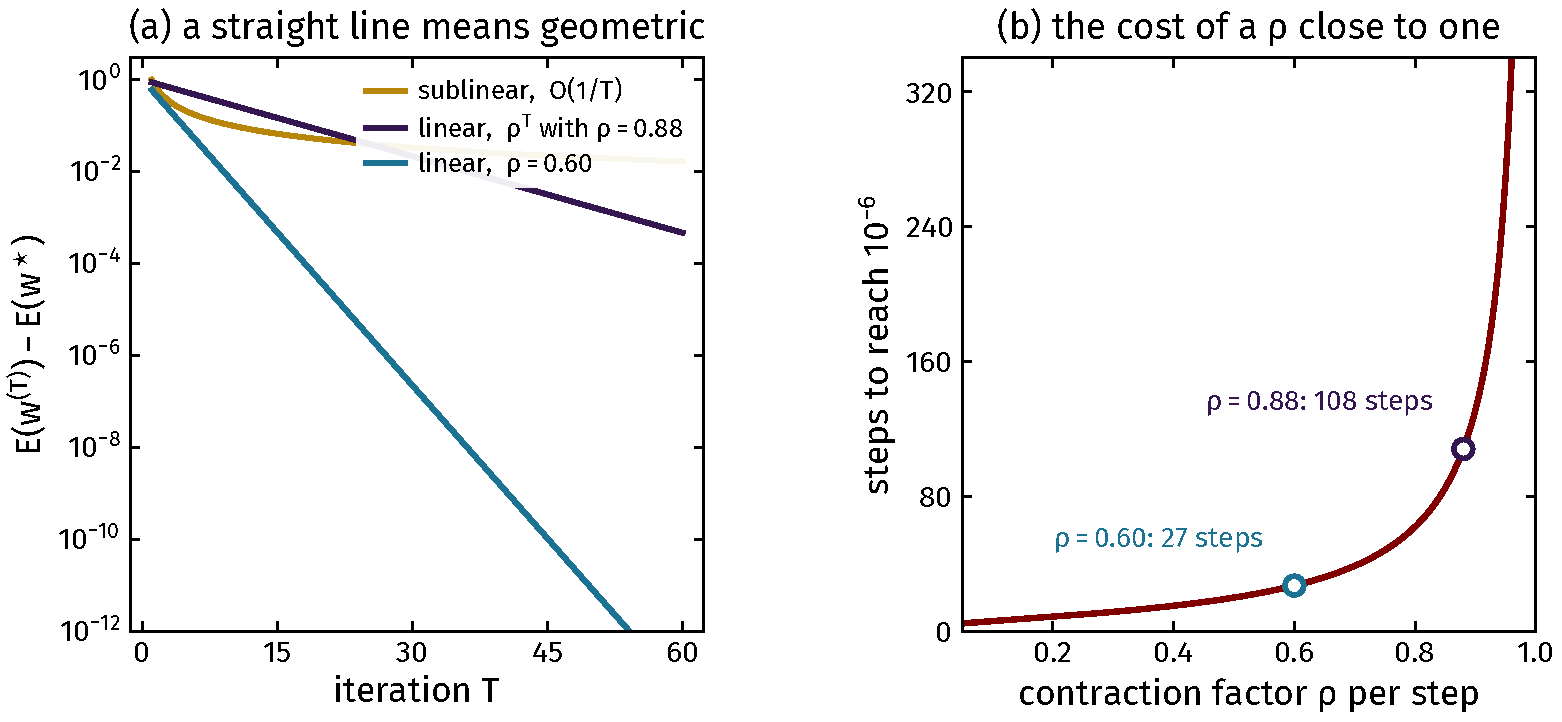
\includegraphics[height=0.545\textheight]{convergence_rates}
  \end{center}
  \figcap[0.97]{(a) error above the optimum against iteration, on a
  logarithmic axis: a geometric rate is a straight line. (b) how many
  steps a given contraction factor needs.}
\end{frame}

\begin{frame}{The tool: the quadratic model, again}
  \bridge{The local quadratic model to say what a minimum
  looks like. The same model now says how the iterate moves on it.}
  \vspace{-0.2em}
  \[
    E(\mathbf{w}) = E(\mathbf{w}^\star) + \tfrac12 \sum_i \lambda_i \alpha_i^2 ,
    \qquad \mathbf{w} - \mathbf{w}^\star = \sum_i \alpha_i \mathbf{u}_i .
  \]
  \vspace{-0.6em}
  \begin{itemize}\itemsep0.35em
    \item $\mathbf{H} \mathbf{u}_i = \lambda_i \mathbf{u}_i$, and the $\mathbf{u}_i$ are orthonormal
    \item $\alpha_i = \mathbf{u}_i^{\mathsf T}(\mathbf{w} - \mathbf{w}^\star)$ is the distance to
          the minimum along $\mathbf{u}_i$
    \item The analysis is exact for a quadratic and a good local
          description near any minimum
  \end{itemize}
  \srcline{Bishop \& Bishop (2024), Eqs.~7.7--7.11.}
\end{frame}

% =====================================================================
\section{The Best Case: Equal Curvature}
% =====================================================================

\begin{frame}{The directions never interact}
  \vspace{-0.25em}
  \begin{lemmax}[Decoupled contraction]\label{th:decay}
    \small
    Apply $\mathbf{w} \leftarrow \mathbf{w} - \eta \nabla E$ to the quadratic model. Then
    each coefficient evolves independently,
    \[
      \alpha_i^{\text{new}} = (1 - \eta\lambda_i)\,\alpha_i^{\text{old}},
      \qquad\text{so}\qquad
      \alpha_i^{(T)} = (1 - \eta\lambda_i)^{T}\,\alpha_i^{(0)} .
    \]
  \end{lemmax}
  \vspace{0.05em}
  {\footnotesize
  \begin{itemize}\itemsep0.26em
    \item \focus{1}{Differentiating the model gives
          $\nabla E = \sum_i \lambda_i \alpha_i \mathbf{u}_i$.}
    \item \focus{1}{Write the update in the same basis,
          $\Delta \mathbf{w} = \sum_i \Delta\alpha_i \mathbf{u}_i$.}
    \item \focus{1}{Matching coefficients in
          $\Delta \mathbf{w} = -\eta\nabla E$ and using $\mathbf{u}_i^{\mathsf T}\mathbf{u}_j =
          \delta_{ij}$ gives $\Delta\alpha_i = -\eta\lambda_i\alpha_i$.}
    \item \focus{1}{Iterating that one-line recursion $T$ times gives
          the stated power. \hfill $\square$}
  \end{itemize}}
  \vspace{-0.3em}
  \srcline{Bishop \& Bishop (2024), Eqs.~7.24--7.29.}
\end{frame}

\begin{frame}{One learning rate, many curvatures}
  \begin{center}
    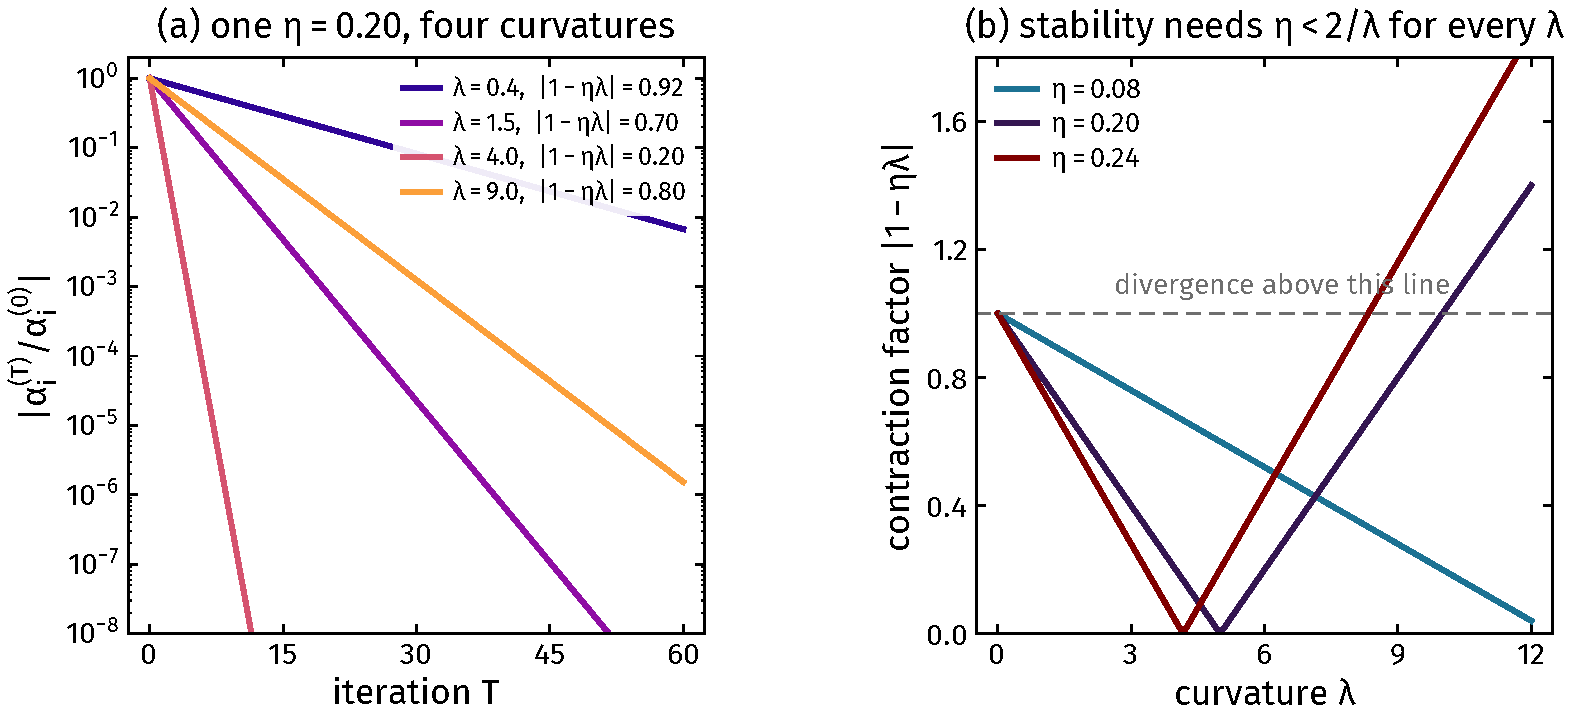
\includegraphics[height=0.545\textheight]{eigen_decay}
  \end{center}
  \figcap[0.97]{(a) the four contraction factors a single $\eta$
  produces on four curvatures. (b) $|1 - \eta\lambda|$ must stay below
  one for \emph{every} eigenvalue}
\end{frame}

\begin{frame}{What that recursion already tells us}
  \vspace{-0.2em}
  \vspace{-0.3em}
  \begin{corx}[Stability and linear convergence]\label{th:stab}
    \small
    The iteration reaches $\mathbf{w}^\star$ if and only if
    $|1 - \eta\lambda_i| < 1$ for every $i$, that is
    $0 < \eta < 2/\lambda_{\max}$, and it then converges
    \alert{linearly} with $\rho = \max_i |1 - \eta\lambda_i|$ in the neighborhood of $\mathbf{w}^\star$.
  \end{corx}
  \vspace{0.3em}
  \begin{itemize}\itemsep0.35em
    \item  $\eta < 2/L$ from smoothness; on a quadratic
          $L = \lambda_{\max}$, and the two agree exactly
    \item $1 - \eta\lambda_i$ may go \alert{negative}: that is
          oscillation, harmless while the magnitude stays below one
    \item Convergence also needs every $\lambda_i > 0$, so the stationary
          point really is a minimum
  \end{itemize}
  \srcline{Bishop \& Bishop (2024), \S7.3.}
\end{frame}

\begin{frame}{When every direction curves alike}
  \begin{center}
    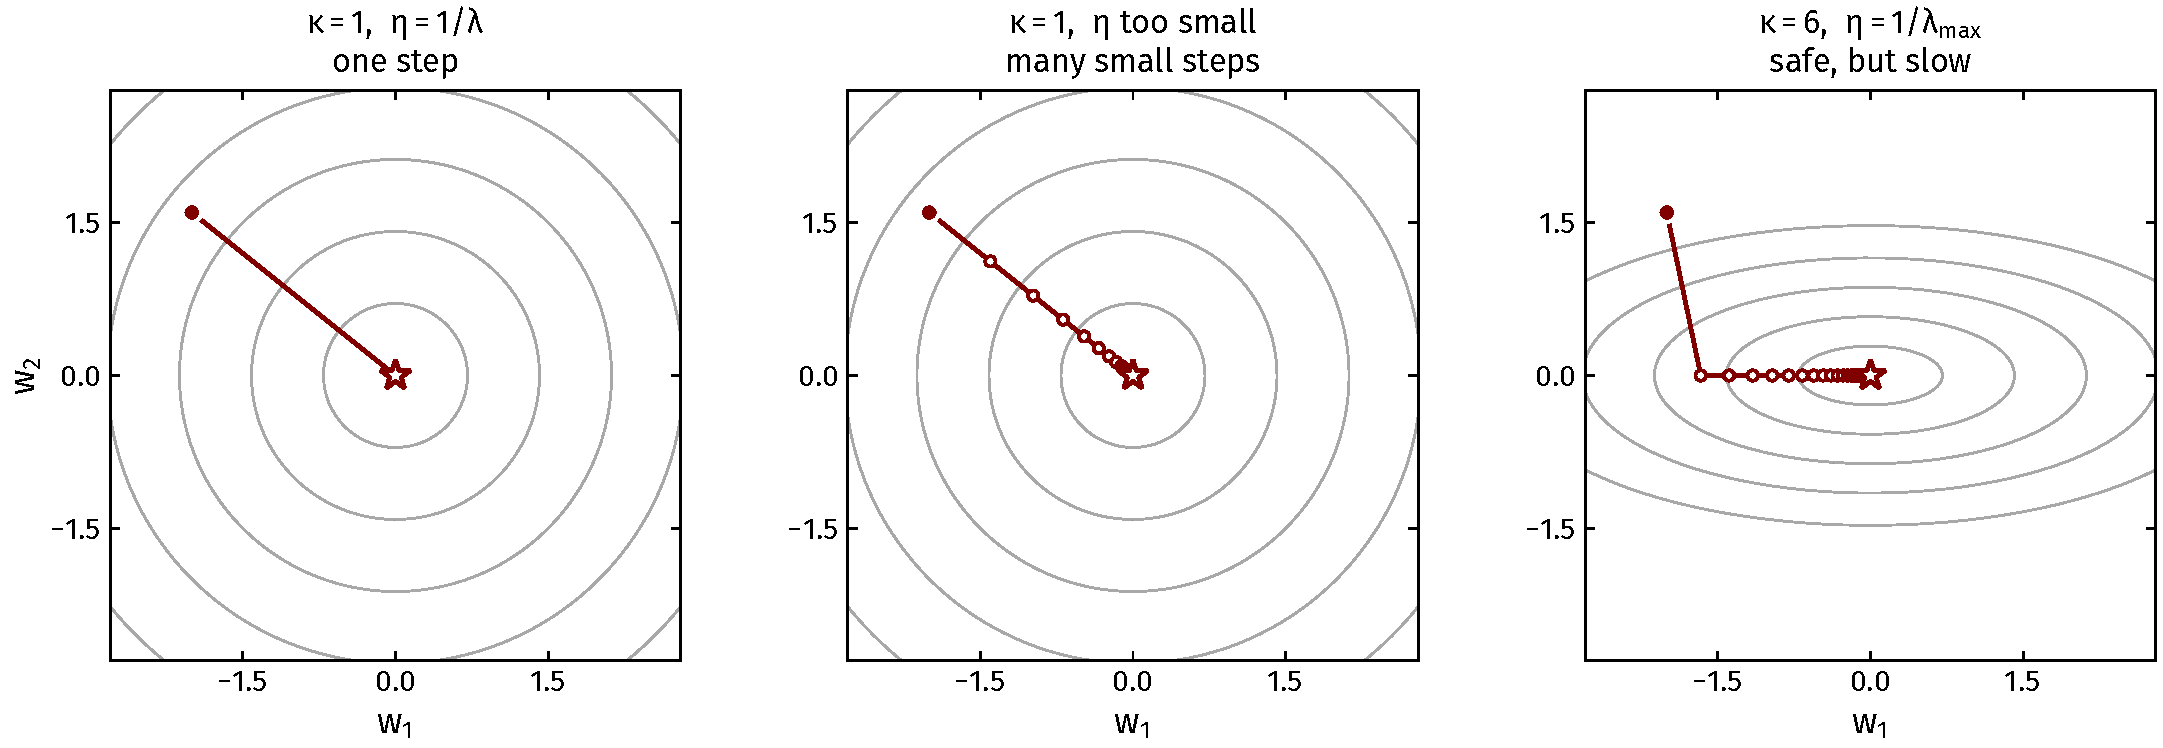
\includegraphics[width=0.98\linewidth]{well_conditioned}
  \end{center}
  \figcap[0.98]{With $\lambda_1 = \lambda_2,\,
      \kappa \;=\; \frac{\lambda_{\max}}{\lambda_{\min}}$ the contours are circles,
  the negative gradient points straight at the minimum, and
  $\eta = 1/\lambda$ arrives in a single step. The last panel shows what
  a modest spread of curvature already costs.}
\end{frame}

% \begin{frame}{The best case, stated}
%   \vspace{0.3em}
%   \begin{itemize}\itemsep0.45em
%     \item If all $\lambda_i$ are equal then $\eta = 1/\lambda$ makes
%           every factor $1 - \eta\lambda_i$ exactly zero
%     \item One step. $\rho = 0$. No method in the rest of this class
%           improves on it
%     \item The reason is that $\mathbf{H} = \lambda I$, so $-\nabla E$ points
%           \alert{exactly} at the minimum from everywhere
%   \end{itemize}
%   \vspace{0.6em}
%   \begin{redhighlight}
%     Everything that follows exists because real error surfaces do not
%     have equal curvature in every direction. The rest of this class
%     measures that failure and repairs it.
%   \end{redhighlight}
% \end{frame}

% =====================================================================
\section{Ill-conditioning}
% =====================================================================

\begin{frame}{The condition number}
  \begin{block}{Definition (condition number of the Hessian)}
    \[
      \kappa \;=\; \frac{\lambda_{\max}}{\lambda_{\min}} \;\geq\; 1 .
    \]
    A problem with large $\kappa$ is called \alert{ill-conditioned}.
  \end{block}
  \vspace{0.4em}
  \begin{itemize}\itemsep0.4em
    \item $\kappa = 1$ is the circular bowl of the previous section
    \item Geometrically, $\sqrt{\kappa}$ is the ratio of the longest to
          the shortest semi-axis of a contour ellipse
    \item $\lambda_{\max}$ limits how large $\eta$ may be;
          $\lambda_{\min}$ limits how fast the slowest direction moves.
          One number cannot satisfy both
  \end{itemize}
  \srcline{Bishop \& Bishop (2024), \S7.3.}
\end{frame}

\begin{frame}{The condition number as the shape of a contour}
  \vspace{-0.1em}
  A contour of the quadratic model is the set
  $\tfrac12\sum_i \lambda_i \alpha_i^2 = c$, where
  $\alpha_i = \mathbf{u}_i^{\mathsf T}(\mathbf{w}-\mathbf{w}^\star)$.
  That is an \alert{ellipse}: its axes point along the eigenvectors
  $\mathbf{u}_i$, and the semi-axis along $\mathbf{u}_i$ has length
  \[
    a_i \;=\; \sqrt{2c}\,\lambda_i^{-1/2}
    \qquad\Longrightarrow\qquad
    \frac{a_{\max}}{a_{\min}}
      \;=\; \sqrt{\frac{\lambda_{\max}}{\lambda_{\min}}}
      \;=\; \sqrt{\kappa}.
  \]
  \vspace{-0.4em}
  \begin{itemize}\itemsep0.35em
    \item  Large $\lambda$, small $\lambda^{-1/2}$ gives the \emph{short} axis
          
    \item $\kappa$ is therefore the elongation of the contour, squared
  \end{itemize}
  \srcline{Bishop \& Bishop (2024), Eqs.~7.10--7.14.}
\end{frame}

\begin{frame}{Why the shape matters for descent}
  \begin{center}
    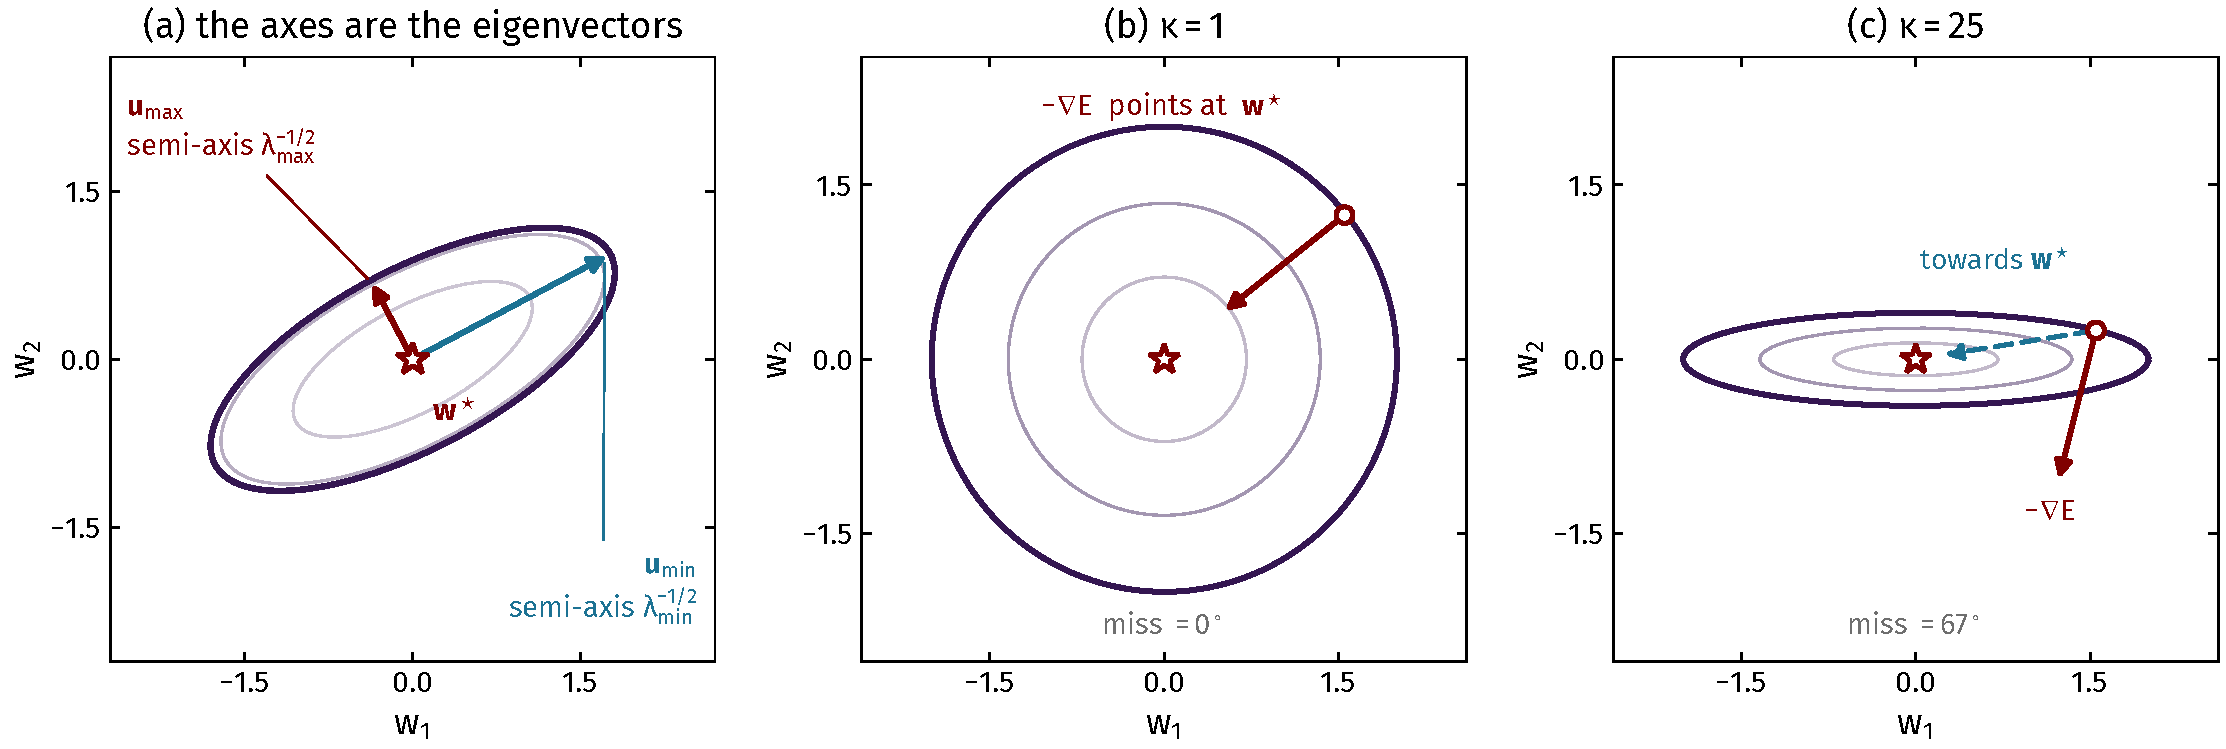
\includegraphics[height=0.49\textheight]{ellipse_geometry}
  \end{center}
  \figcap[0.97]{(a) the semi-axes of one contour, named. (b) on a
  circular contour the negative gradient points exactly at
  $\mathbf{w}^\star$. (c) on an elongated contour it misses by a wide
  angle, and the step spends most of its length crossing the valley
  rather than travelling along it.}
\end{frame}

% \begin{frame}{What ill-conditioning costs}
%   \begin{center}
%     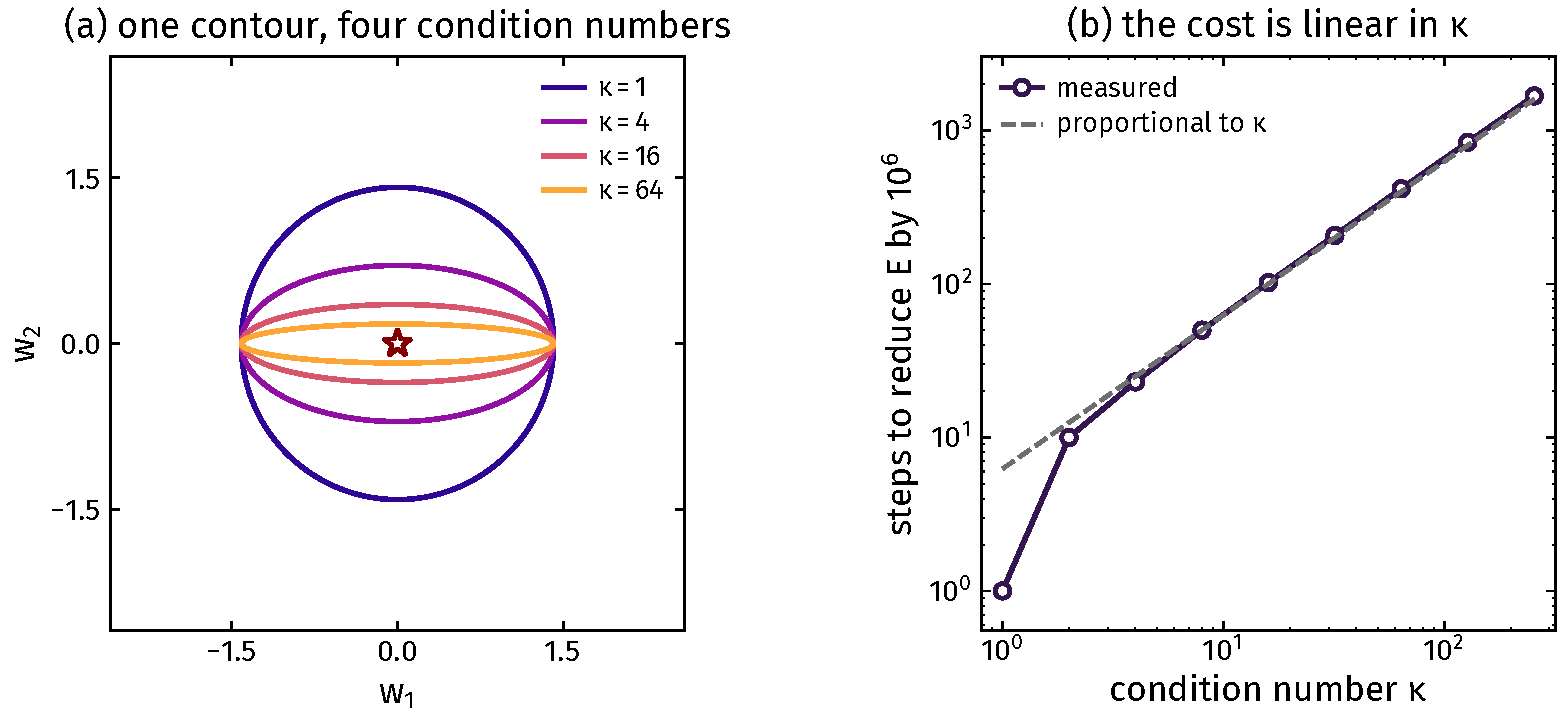
\includegraphics[height=0.58\textheight]{condition_number}
%   \end{center}
%   \figcap[0.97]{(a) Four condition
%   numbers and minimum. (b) steps needed to reduce the error by six orders of
%   magnitude, at the largest safe learning rate, against $\kappa$: the
%   count grows in proportion to $\kappa$.}
% \end{frame}

\begin{frame}{The slowest direction sets the pace}
  \vspace{-0.2em}
  \begin{propx}[The rate at the stability limit]\label{th:slow}
    \small
    Take $\eta$ as large as stability allows,
    $\eta \to 2/\lambda_{\max}$. Then, the rate of convergence is dominated by $\lambda_{min}$ and
    \[
      \Big| 1 - \frac{2\lambda_{\min}}{\lambda_{\max}} \Big|
      \;=\; \Big| 1 - \frac{2}{\kappa} \Big|
      \qquad\text{per step.}
    \]
    For large $\kappa$ this is $1 - 2/\kappa$: a factor that approaches
    one as the problem worsens.
  \end{propx}
  \vspace{0.3em}
  \begin{itemize}\itemsep0.35em
    \item Pushing $\eta$ to its limit buys speed in the direction that
          was never the problem; the long axis of the ellipse is the one
          that needs the steps
  \end{itemize}
  \srcline{Bishop \& Bishop (2024), Eq.~7.30.}
\end{frame}

\begin{frame}{Optimal learning rate for a quadratic}
  \vspace{-0.2em}
  \begin{propx}[The optimal learning rate for a quadratic]\label{th:opt}
    \small
        The choice $\eta^\star = 2/(\lambda_{\min} + \lambda_{\max})$
        minimises $\rho = \max_i |1 - \eta\lambda_i|$, giving
        $\rho^\star = (\kappa - 1)/(\kappa + 1)$.
  \end{propx}
  \vspace{0.05em}
  % {\footnotesize
  % \begin{itemize}\itemsep0.26em
  %   \item \focus{1}{$\rho(\eta) = \max\big(|1-\eta\lambda_{\min}|,\,
  %         |1-\eta\lambda_{\max}|\big)$: only the extremes can attain the
  %         maximum.}
  %   \item \focus{1}{The first term falls in $\eta$, the second rises, so
  %         the maximum is smallest where they are equal.}
  %   \item \focus{1}{$1 - \eta\lambda_{\min} = \eta\lambda_{\max} - 1$
  %         gives $\eta^\star = 2/(\lambda_{\min}+\lambda_{\max})$.}
  %   \item \focus{1}{Substituting back gives the stated factor.
  %         \hfill $\square$}
  % \end{itemize}}
  \vspace{-0.4em}
  \begin{redhighlight}
    Accuracy $\epsilon$ then needs about
    $\tfrac{\kappa+1}{2}\ln(1/\epsilon)$ steps: the cost is
    \alert{proportional to $\kappa$}, however cleverly $\eta$ is chosen.
  \end{redhighlight}
\end{frame}

\begin{frame}{The valley}
  \begin{center}
    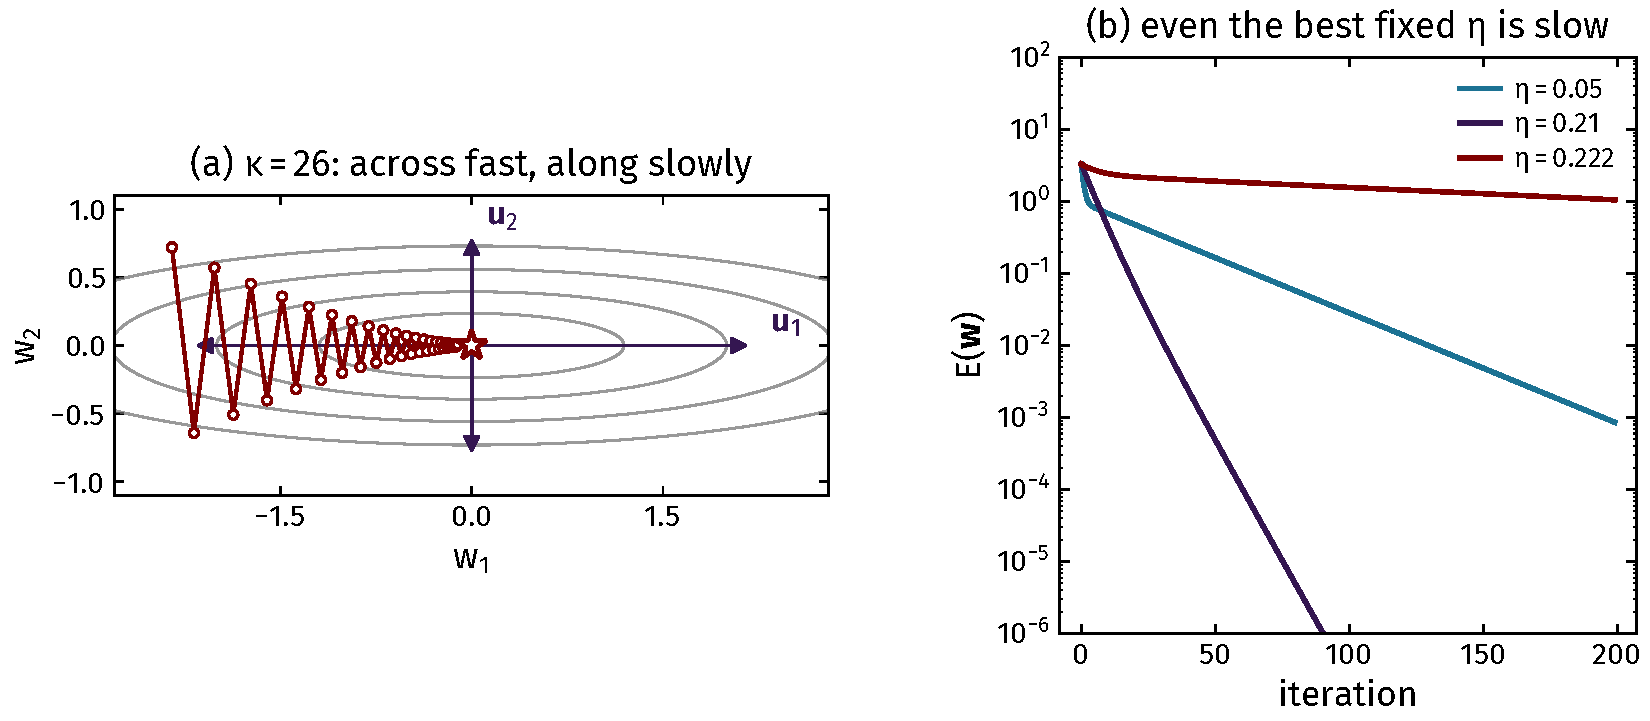
\includegraphics[height=0.58\textheight]{valley}
  \end{center}
  \figcap[0.97]{(a) with $\kappa \approx 26$ the negative gradient points
  almost across the valley rather than along it, so successive steps
  oscillate. (b) three fixed learning rates on that surface: the best of
  them is still slow.}
\end{frame}

\begin{frame}{Possible Origin of Condition Number}
  \vspace{0.1em}
  \begin{itemize}\itemsep0.3em
    \item \alert{Input scale}: a feature measured in millimetres and one
          measured in kilometres produce curvatures differing by $10^{12}$
    \item \alert{Correlated inputs}: two nearly identical features make
          one eigenvalue nearly zero
    \item \alert{Depth}: the same weight change has a different effect
          early and late in a network, so layers differ in curvature by
          orders of magnitude
    \item \alert{Output scale}: an unnormalised target inflates every
          eigenvalue at once
  \end{itemize}
  \vspace{0.25em}
  \begin{redhighlight}
    Two responses are possible. Change the \emph{iteration}, which is the rest of
    this class. Or change the \emph{problem} so that $\kappa$ is small to
    begin with, which is Class 15.
  \end{redhighlight}
\end{frame}

% =====================================================================
\section{Momentum}
% =====================================================================

\begin{frame}{A ball with inertia}
  \vspace{-0.3em}
  \begin{center}
  \begin{tikzpicture}[>=Stealth, font=\scriptsize, scale=0.99,
      ball/.style={circle, draw=dpc, fill=dpc!25, line width=0.9pt,
                   inner sep=0pt, minimum size=5.4pt},
      vel/.style={->, dpc, line width=1.35pt},
      hill/.style={shc, line width=1.3pt}]

    % ================= (a) a long, gentle slope =====================
    \begin{scope}[shift={(0,0)}]
      \fill[shc!10] (0,0.05) -- plot[domain=0:5.8, samples=70, smooth]
            (\x,{2.05*exp(-0.40*\x)}) -- (5.8,0.05) -- cycle;
      \draw[hill, domain=0:5.8, samples=70, smooth]
            plot (\x,{2.05*exp(-0.40*\x)});

      \node[ball] at (0.60,1.78) {};
      \draw[vel] (0.60,1.78) -- (1.06,1.48);
      \node[ball] at (1.90,1.13) {};
      \draw[vel] (1.90,1.13) -- (2.69,0.82);
      \node[ball] at (3.20,0.74) {};
      \draw[vel] (3.20,0.74) -- (4.37,0.47);
      \node[ball] at (4.50,0.51) {};
      \draw[vel] (4.50,0.51) -- (5.90,0.32);

      \node[dpc, above=0pt] at (0.88,1.61) {$v_1$};
      \node[dpc, above=0pt] at (2.32,0.96) {$v_2$};
      \node[dpc, above=0pt] at (3.82,0.59) {$v_3$};

      \node[shc, font=\footnotesize] at (2.9,2.72)
        {\textbf{(a) a long, gentle slope}};
      \node[mcMuted, align=center] at (2.9,-0.50)
        {the slope pushes the same way each time,\\
         so the pushes \emph{add}};
      \node[dpc, font=\footnotesize] at (2.9,-1.40)
        {$v_1 < v_2 < v_3$:\; the ball builds speed};
    \end{scope}

    % ================= (b) a narrow gully ===========================
    \begin{scope}[shift={(7.4,0)}]
      \fill[shc!10] (0.85,0.05) -- plot[domain=0.85:4.55, samples=70,
            smooth] (\x,{0.62*(\x-2.7)*(\x-2.7)}) -- (4.55,0.05) -- cycle;
      \draw[hill, domain=0.85:4.55, samples=70, smooth]
            plot (\x,{0.62*(\x-2.7)*(\x-2.7)});
      \draw[mcMuted, dashed, line width=0.7pt] (2.70,-0.05) -- (2.70,2.30);

      \node[ball] at (1.05,1.87) {};
      \draw[vel] (1.05,1.87) -- (1.38,1.20);
      \node[ball] at (4.30,1.93) {};
      \draw[vel] (4.30,1.93) -- (4.00,1.34);
      \node[ball] at (1.98,0.56) {};
      \draw[vel] (1.98,0.56) -- (2.34,0.24);

      \node[dpc, above left=-3pt and -2pt] at (1.05,1.87) {\textbf{1}};
      \node[dpc, above right=-3pt and -2pt] at (4.30,1.93) {\textbf{2}};
      \node[dpc, below left=-2pt and -2pt] at (1.98,0.56) {\textbf{3}};

      \node[shc, font=\footnotesize] at (2.7,2.72)
        {\textbf{(b) a narrow gully}};
      \node[mcMuted, align=center] at (2.7,-0.50)
        {the slope reverses at every crossing,\\
         so the pushes \emph{cancel}};
      \node[dpc, font=\footnotesize] at (2.7,-1.40)
        {the sideways swing dies away};
    \end{scope}
  \end{tikzpicture}
  \end{center}
  \vspace{-0.1em}
  \begin{redhighlight}
    The same rule does both: it accelerates where the slope is
    consistent and stays out of the way where it alternates.
  \end{redhighlight}
\end{frame}

\begin{frame}{The analogy, term by term}
  \vspace{0.45em}
  {\footnotesize
  \renewcommand{\arraystretch}{1.42}
  \begin{tabular}{@{}l@{\hspace{2.2em}}l@{}}
    \textbf{A ball rolling downhill} & \textbf{In the update}\\
    it keeps some of its previous velocity & $\mu\,\Delta \mathbf{w}^{(\tau-2)}$\\
    the slope adds to that velocity & $-\eta\nabla E$\\
    a long consistent slope builds speed & aligned gradients accumulate\\
    a narrow gully cancels sideways motion & alternating gradients
      cancel\\
  \end{tabular}}
  \vspace{1.0em}

  \begin{itemize}\itemsep0.4em
    \item A ball does not stop and re-measure the slope at every
          instant, and neither should the iterate
    \item The single parameter $\mu$ decides how much of the past to
          keep
  \end{itemize}
\end{frame}

\begin{frame}{The momentum update}
  \vspace{-0.3em}
  \[
    \Delta \mathbf{w}^{(\tau-1)}
      \;=\; -\eta\,\nabla E\!\left(\mathbf{w}^{(\tau-1)}\right)
            \;+\; \mu\,\Delta \mathbf{w}^{(\tau-2)},
    \qquad
    \mathbf{w}^{(\tau)} = \mathbf{w}^{(\tau-1)} + \Delta \mathbf{w}^{(\tau-1)}
  \]
  \vspace{-0.7em}
  \begin{itemize}\itemsep0.35em
    \item $\mu \in [0, 1)$; a typical value is $0.9$
    \item Unrolling the recursion shows $\Delta \mathbf{w}$ is an exponentially
          weighted sum of \alert{every} past gradient
    \item Prince writes the same idea as a running average,
          $m \leftarrow \beta m + (1-\beta)\nabla E$ and
          $\mathbf{w} \leftarrow \mathbf{w} - \eta \mathbf{m}$, which rescales $\eta$ by
          $(1-\beta)$ but is otherwise identical
  \end{itemize}
  \srcline{Bishop \& Bishop (2024), Eq.~7.31; Prince (2023), Eq.~6.11.}
\end{frame}

\begin{frame}{Why momentum helps where it helps}
  \vspace{-0.25em}
  \begin{propx}[Effective learning rate on a consistent slope]\label{th:mom}
    \small
    If the gradient is essentially unchanged over a long run of steps,
    the momentum update converges to
    \[
      \Delta \mathbf{w} \;=\; -\eta\,\nabla E\,\{1 + \mu + \mu^2 + \cdots\}
                \;=\; -\frac{\eta}{1-\mu}\,\nabla E ,
    \]
    so the effective learning rate is $\eta/(1-\mu)$. With $\mu = 0.9$
    that is a tenfold increase.
  \end{propx}
  \vspace{0.3em}
  \begin{itemize}\itemsep0.35em
    \item Where successive gradients \alert{alternate} in sign the terms
          cancel instead, and the effective rate stays near $\eta$
    \item That asymmetry is the whole mechanism: acceleration along the
          valley, no amplification across it
  \end{itemize}
  \srcline{Bishop \& Bishop (2024), Eqs.~7.32--7.33.}
\end{frame}

\begin{frame}{The two regimes}
  \begin{center}
    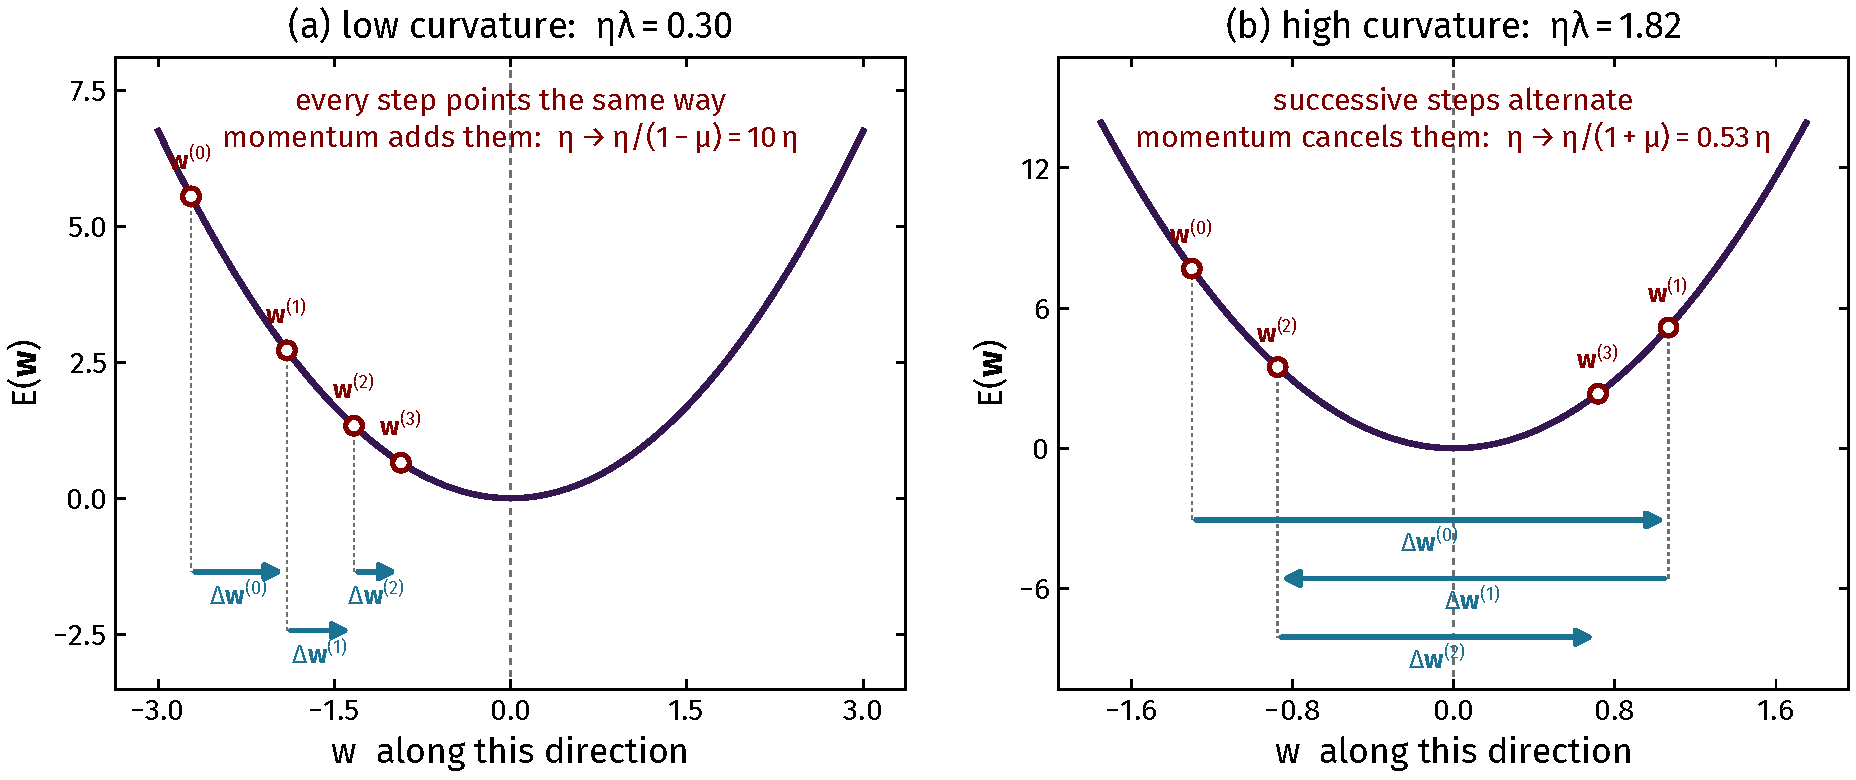
\includegraphics[height=0.50\textheight]{momentum_regimes}
  \end{center}
  \figcap[0.97]{Plain gradient descent at one fixed $\eta$, along two
  directions of the same surface. (a) low curvature: the displacements
  $\Delta \mathbf{w}^{(k)}$ all point the same way. (b) high curvature: the
  same $\eta$ overshoots, so they alternate.}
  \srcline{Following the geometry of Bishop \& Bishop (2024),
  Figs.~7.4 and 7.5.}
\end{frame}

\begin{frame}{The same two regimes, measured}
  \begin{center}
    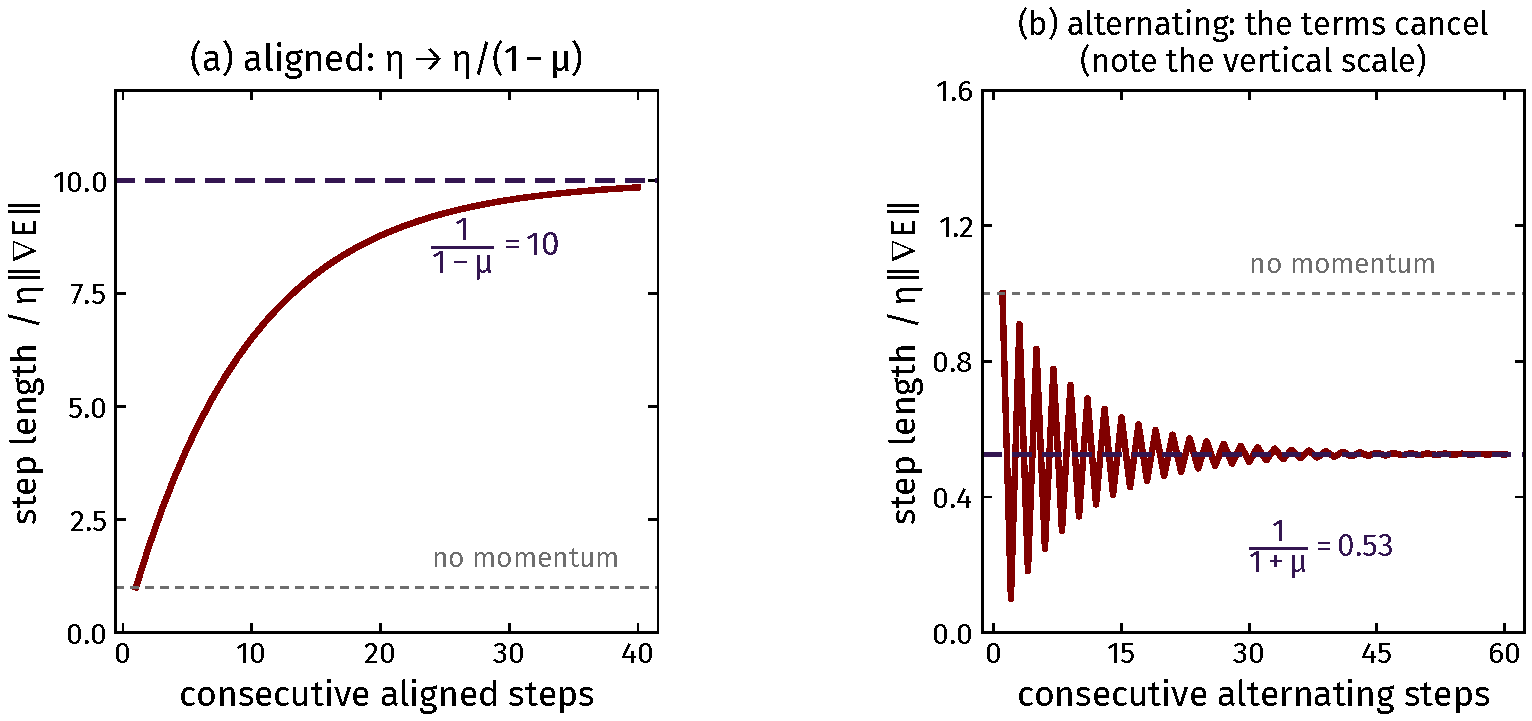
\includegraphics[height=0.545\textheight]{momentum_multiplier}
  \end{center}
  \figcap[0.97]{The length of the accumulated step, in units of
  $\eta\|\nabla E\|$. (a) with the gradient pointing the same way each
  time it approaches $1/(1-\mu)$. (b) with the gradient alternating it
  settles near $1/(1+\mu)$ --- below one, not above.}
\end{frame}

% \begin{frame}{Momentum on the valley}
%   \begin{center}
%     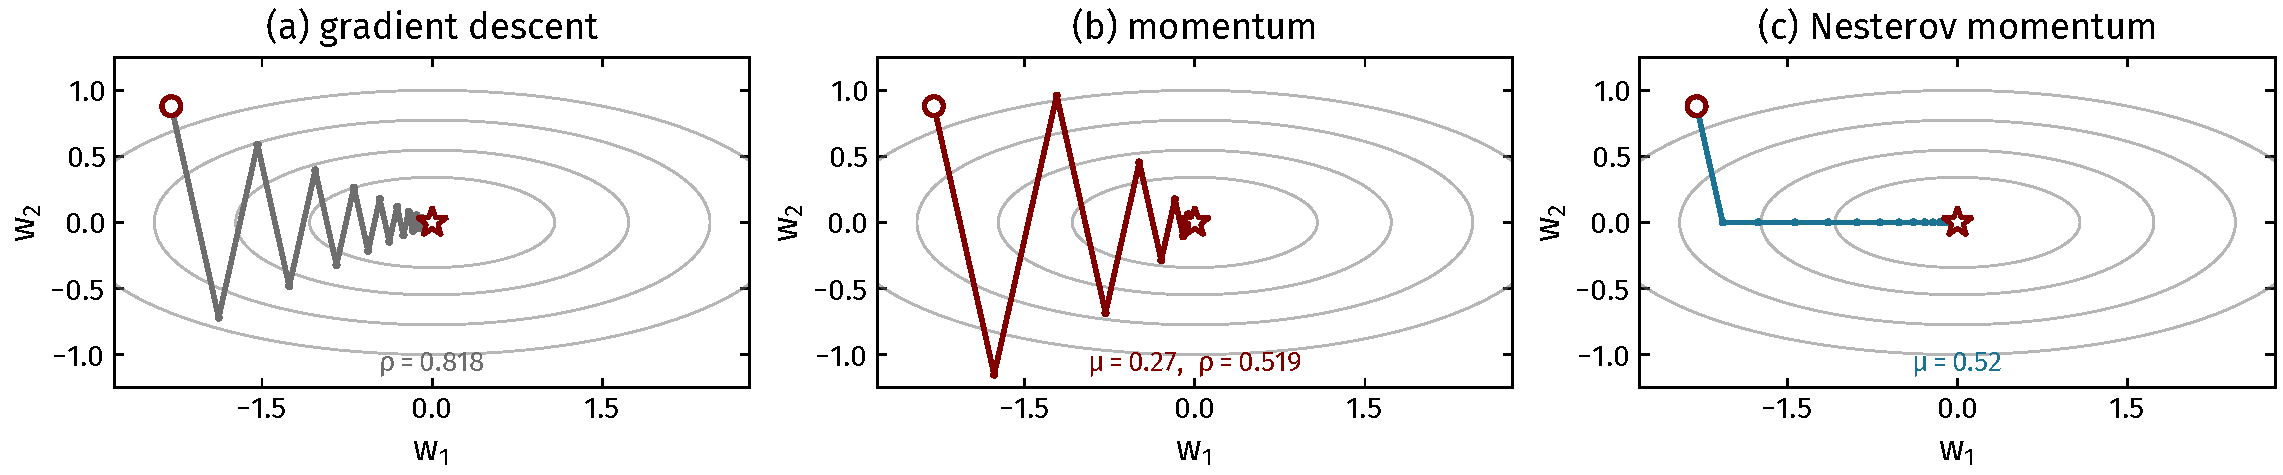
\includegraphics[width=0.94\linewidth]{momentum_paths}
%   \end{center}
%   \figcap[0.97]{The same surface and start, each method at the constants
%   that are optimal for it; the first twenty iterates are marked. Momentum
%   crosses the valley fewer times and travels much further along it per
%   step, and the contraction factor falls from $0.818$ to $0.519$.}
% \end{frame}
\begin{frame}{Nesterov momentum}
  \vspace{-0.9em}
  \[
    \Delta \mathbf{w}^{(\tau-1)}
      = -\eta\,\nabla E\!\left(\mathbf{w}^{(\tau-1)}
                              + \mu\,\Delta \mathbf{w}^{(\tau-2)}\right)
        + \mu\,\Delta \mathbf{w}^{(\tau-2)}
  \]
  \vspace{-0.2em}
  \begin{itemize}\itemsep0.4em
    \item The two ingredients are unchanged: a momentum carry
          $\mu\,\Delta \mathbf{w}^{(\tau-2)}$ and a gradient step $-\eta\nabla E$
    \item Only the \alert{order} changes. Classical momentum measures
          the slope where the iterate is; Nesterov carries first and
          measures the slope where it is about to be
    \item Because the look-ahead point is already past the turn, the
          gradient measured there points back, and the overshoot is
          corrected within the same step
  \end{itemize}
  \srcline{Bishop \& Bishop (2024), Eq.~7.34; Prince (2023), Eq.~6.12.}
\end{frame}

\begin{frame}{Nesterov on the same valley}
  \begin{center}
    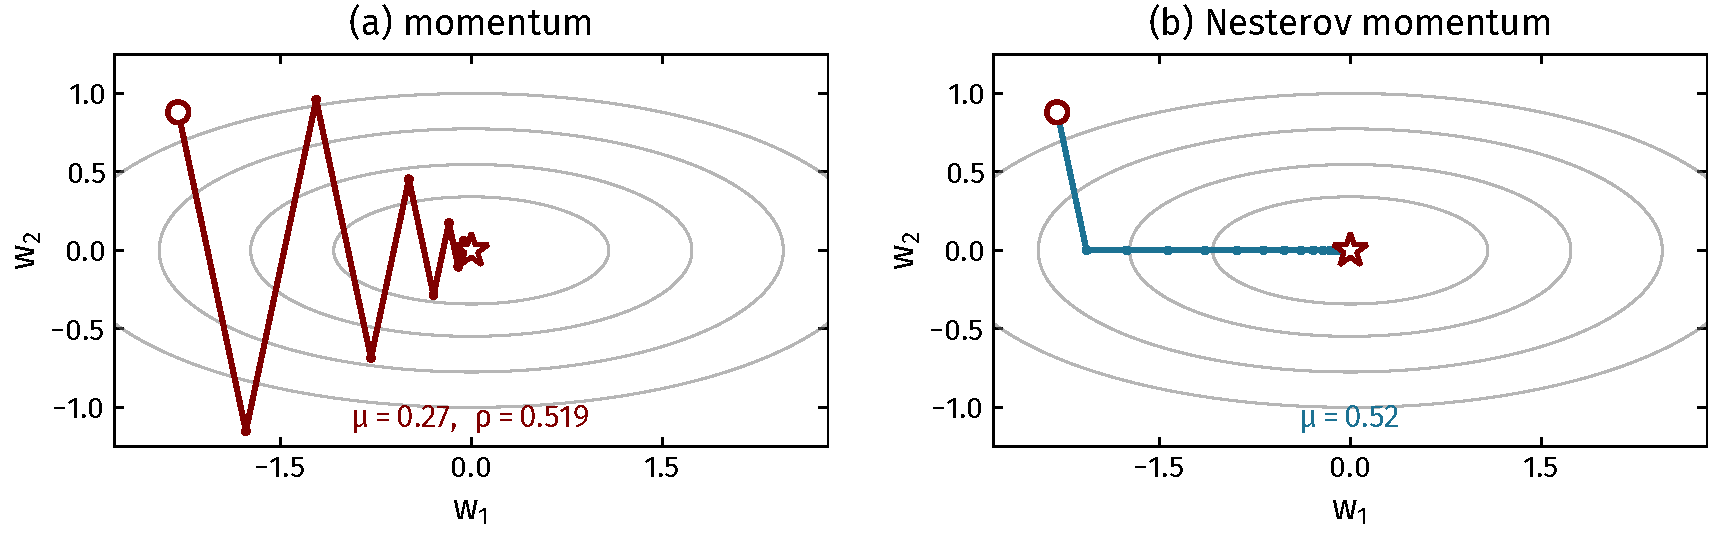
\includegraphics[width=0.94\linewidth]{nesterov_path}
  \end{center}
  \figcap[0.97]{Momentum repeated on the left as the reference. Nesterov
  removes the crossing of the valley in a single step and then runs
  straight along the floor, because the gradient is measured at the
  look-ahead point rather than at the current one.}
\end{frame}

\begin{frame}{What that costs in iterations}
  \begin{center}
    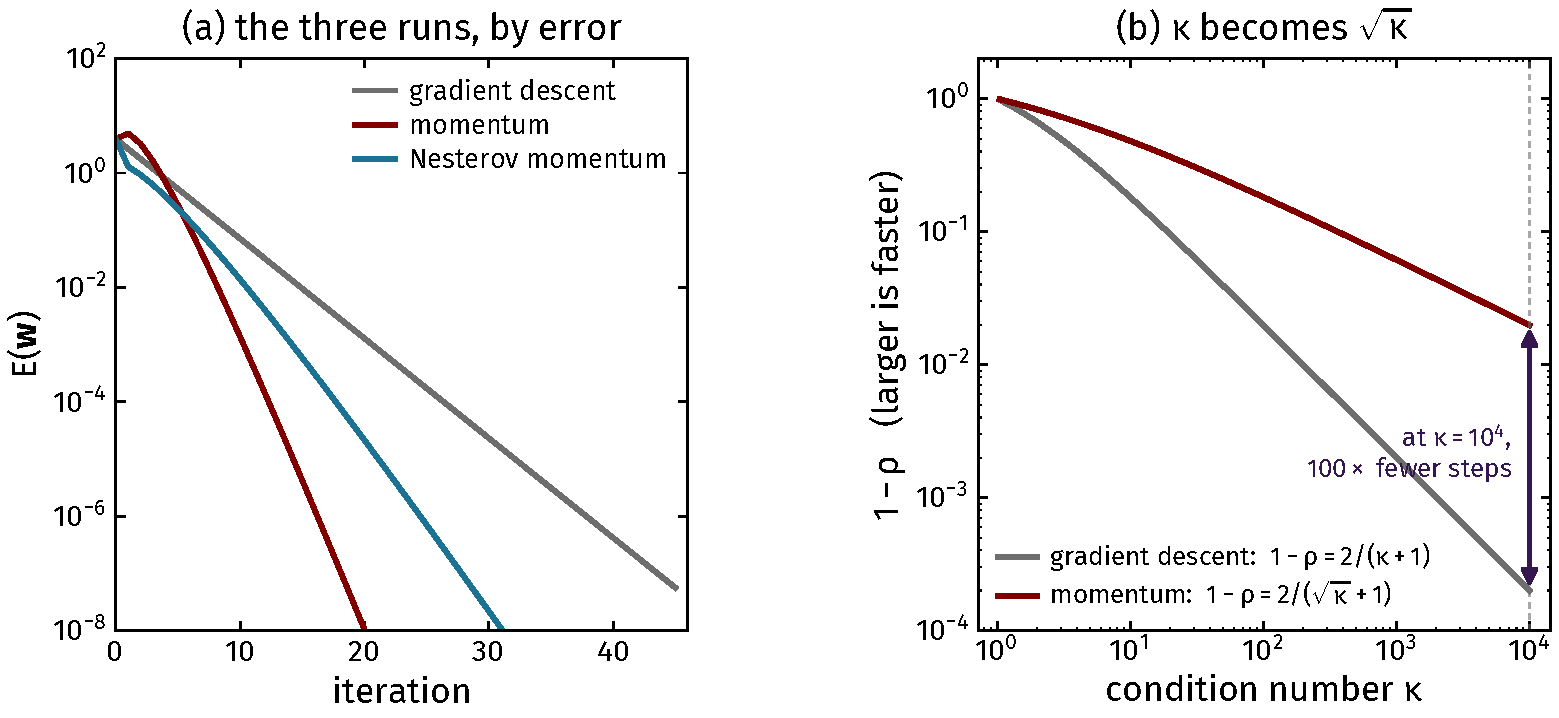
\includegraphics[height=0.545\textheight]{momentum_error}
  \end{center}
  \figcap[0.97]{(a) the three runs by error, on a logarithmic axis,
  where a geometric rate is a straight line. (b) the two contraction
  factors against $\kappa$: gradient descent loses a factor $\kappa$,
  momentum only $\sqrt{\kappa}$.}
\end{frame}

\begin{frame}{Momentum: }
  \vspace{-0.2em}
  \begin{propx}[Heavy-ball acceleration on a quadratic]\label{th:hb}
    \small
    On a quadratic function with condition number $\kappa$, the choices
    $\mu^\star = \big((\sqrt{\kappa}-1)/(\sqrt{\kappa}+1)\big)^{2}$ and
    $\eta^\star = 4/(\sqrt{\lambda_{\max}}+\sqrt{\lambda_{\min}})^{2}$
    give a contraction factor
    $\rho = (\sqrt{\kappa}-1)/(\sqrt{\kappa}+1)$.
  \end{propx}
  \vspace{0.3em}
  \begin{propx}[The optimal learning rate for a quadratic]\label{th:opt}
    \small
        The choice $\eta^\star = 2/(\lambda_{\min} + \lambda_{\max})$
        minimises $\rho = \max_i |1 - \eta\lambda_i|$, giving
        $\rho^\star = (\kappa - 1)/(\kappa + 1)$.
  \end{propx}
  \begin{itemize}\itemsep0.3em
    \item Compare Proposition~\ref{th:opt}: $\kappa$ has become
          $\sqrt{\kappa}$, so $\kappa = 10^4$ needs $100$ times fewer
          steps
    \item The price is a second hyperparameter, and a trajectory that
          overshoots before it settles
  \end{itemize}
  \srcline{Polyak (1964).}
\end{frame}


\begin{frame}{Nesterov momentum, one step drawn}
  \vspace{-0.7em}
  \begin{center}
  \begin{tikzpicture}[>=Stealth, font=\scriptsize, scale=1.05,
      pa/.style={circle, fill=shc,   inner sep=2.1pt},
      pb/.style={circle, fill=dpc,   inner sep=2.1pt},
      pc/.style={circle, fill=tealc, inner sep=2.1pt},
      cls/.style={->, dpc,   line width=1.3pt},
      nes/.style={->, tealc, line width=1.3pt},
      val/.style={mcMuted, line width=0.6pt}]

    % ================= (a) classical momentum ========================
    \begin{scope}
      \draw[val, rotate around={-16:(2.60,-0.15)}]
        (2.60,-0.15) ellipse (1.05 and 0.44);
      \node[dpc] at (2.60,-0.15) {$\star$};
      \node[mcMuted, right=1pt] at (2.72,-0.18) {$\mathbf{w}^\star$};

      \draw[mcMuted, dashed, line width=0.8pt] (-1.00,2.92) -- (0.20,2.60);
      \node[pa] (a1) at (0.20,2.60) {};
      \node[shc, above right=-3pt and -2pt of a1] {\textbf{1}};

      \draw[cls] (0.20,2.60) -- (1.20,1.10);
      \node[dpc, left=1pt, align=right] at (0.62,1.90)
        {$-\eta\nabla E$\\ at \textbf{1}};
      \node[pb] (a2) at (1.20,1.10) {};
      \node[dpc, left=2pt of a2] {\textbf{2}};

      \draw[cls] (1.20,1.10) -- (3.30,0.45);
      \node[dpc, below=1pt] at (2.10,0.74) {$+\,\mu\Delta \mathbf{w}^{(\tau-2)}$};
      \node[pb] (a3) at (3.30,0.45) {};
      \node[dpc, right=2pt of a3] {\textbf{3}};

      \draw[dpc, line width=0.7pt, dashed] (3.30,0.45) -- (2.60,-0.15);

      \node[shc, font=\footnotesize] at (1.5,3.55)
        {\textbf{(a) classical momentum}};
      \node[dpc] at (1.5,3.12) {measure here, then coast};
    \end{scope}

    % ================= (b) Nesterov momentum =========================
    \begin{scope}[shift={(5.6,0)}]
      \draw[val, rotate around={-16:(2.60,-0.15)}]
        (2.60,-0.15) ellipse (1.05 and 0.44);
      \node[dpc] at (2.60,-0.15) {$\star$};
      \node[mcMuted, right=1pt] at (2.72,-0.18) {$\mathbf{w}^\star$};

      \draw[mcMuted, dashed, line width=0.8pt] (-1.00,2.92) -- (0.20,2.60);
      \node[pa] (b1) at (0.20,2.60) {};
      \node[shc, above right=-3pt and -2pt of b1] {\textbf{1}};

      \draw[nes] (0.20,2.60) -- (2.30,1.95);
      \node[tealc, below=2.5pt] at (1.12,2.22) {$+\,\mu\Delta \mathbf{w}^{(\tau-2)}$};
      \node[pc] (b4) at (2.30,1.95) {};
      \node[tealc, above right=-3pt and -2pt of b4] {\textbf{4}};

      \draw[nes] (2.30,1.95) -- (2.65,0.15);
      \node[tealc, right=2pt, align=left] at (2.72,1.08)
        {$-\eta\nabla E$\\ at \textbf{4}};
      \node[pc] (b5) at (2.65,0.15) {};
      \node[tealc, left=2pt of b5] {\textbf{5}};

      \draw[tealc, line width=0.7pt, dashed] (2.65,0.15) -- (2.60,-0.15);

      \node[shc, font=\footnotesize] at (1.5,3.55)
        {\textbf{(b) Nesterov momentum}};
      \node[tealc] at (1.5,3.12) {coast first, then measure \emph{there}};
    \end{scope}
  \end{tikzpicture}
  \end{center}
  \vspace{-0.35em}
  \begin{redhighlight}
    Both steps use the same two vectors. Taking the carry first puts the
    gradient measurement past the turn, so point \textbf{5} lands nearer
    $\mathbf{w}^\star$ than point \textbf{3}.
  \end{redhighlight}
\end{frame}

\begin{frame}{The guarantee behind the name}
  \vspace{-0.2em}
  \begin{propx}[Accelerated rates]\label{th:nest}
    \small
    For an $L$-smooth convex $E$, Nesterov's method attains
    $E(\mathbf{w}^{(T)}) - E(\mathbf{w}^\star) = O(1/T^{2})$, against $O(1/T)$ for plain
    gradient descent. If $E$ is in addition strongly convex with
    condition number $\kappa$, the contraction factor is
    $1 - 1/\sqrt{\kappa}$ rather than $1 - 1/\kappa$.
  \end{propx}
  \vspace{0.4em}
  \begin{itemize}\itemsep0.4em
    \item No first-order method can do better than $O(1/T^2)$ using only
          gradients, so this is optimal in that class
    \item For \alert{batch} gradient descent the improvement is real;
          with mini-batch noise it is much less clear-cut
  \end{itemize}
  \srcline{Nesterov (1983, 2004); applied to SGD by Sutskever et
  al.~(2013).}
\end{frame}

% \begin{frame}{Stochastic gradient descent with momentum}
%   \vspace{0.2em}
%   \begin{algox}[SGD with momentum]\label{th:algmom}
%     \small
%     \textbf{Input:} data indexed by $n$; batch size $B$; per-batch error
%     $E_{n:n+B-1}$; learning rate $\eta$; momentum $\mu$; initial $\mathbf{w}$\\[0.35em]
%     $n \leftarrow 1$; \quad $\Delta \mathbf{w} \leftarrow 0$\\
%     \textbf{repeat}\\
%     \hspace{1.4em} $\Delta \mathbf{w} \leftarrow -\eta \nabla E_{n:n+B-1}(\mathbf{w})
%       + \mu \Delta \mathbf{w}$ \hfill \textcolor{mcMuted}{// update term}\\
%     \hspace{1.4em} $\mathbf{w} \leftarrow \mathbf{w} + \Delta \mathbf{w}$
%       \hfill \textcolor{mcMuted}{// weight vector update}\\
%     \hspace{1.4em} $n \leftarrow n + B$\\
%     \hspace{1.4em} \textbf{if} $n > N$ \textbf{then}
%       \; shuffle data; \; $n \leftarrow 1$ \; \textbf{end if}\\
%     \textbf{until} convergence; \quad \textbf{return} $\mathbf{w}$
%   \end{algox}
%   \srcline{Bishop \& Bishop (2024), Algorithm 7.3.}
% \end{frame}

% =====================================================================
\section{Learning-rate Schedules}
% =====================================================================

\begin{frame}{Why a fixed step size cannot finish the job}
  \bridge{Momentum attacks the condition number. It does nothing about
  the noise in a mini-batch gradient.}
  \vspace{0.3em}
  \begin{itemize}\itemsep0.35em
    \item The mini-batch gradient's variance does not shrink as $\mathbf{w}$
          approaches $\mathbf{w}^\star$, so near the minimum the signal vanishes
          while the noise does not
    \item The iterate then wanders in a ball whose radius is set by
          $\eta$; halving $\eta$ halves the radius but never removes it
    \item Large $\eta$ explores, small $\eta$ refines --- we want both,
          in that order
  \end{itemize}
  \begin{redhighlight}
    So make $\eta$ a function of the step index:
    $\mathbf{w}^{(\tau)} = \mathbf{w}^{(\tau-1)}
     - \eta^{(\tau-1)}\nabla E_n(\mathbf{w}^{(\tau-1)})$.
  \end{redhighlight}
  \srcline{Bishop \& Bishop (2024), Eq.~7.35; Prince (2023), \S6.2.2.}
\end{frame}

\begin{frame}{The noise floor}
  \begin{center}
    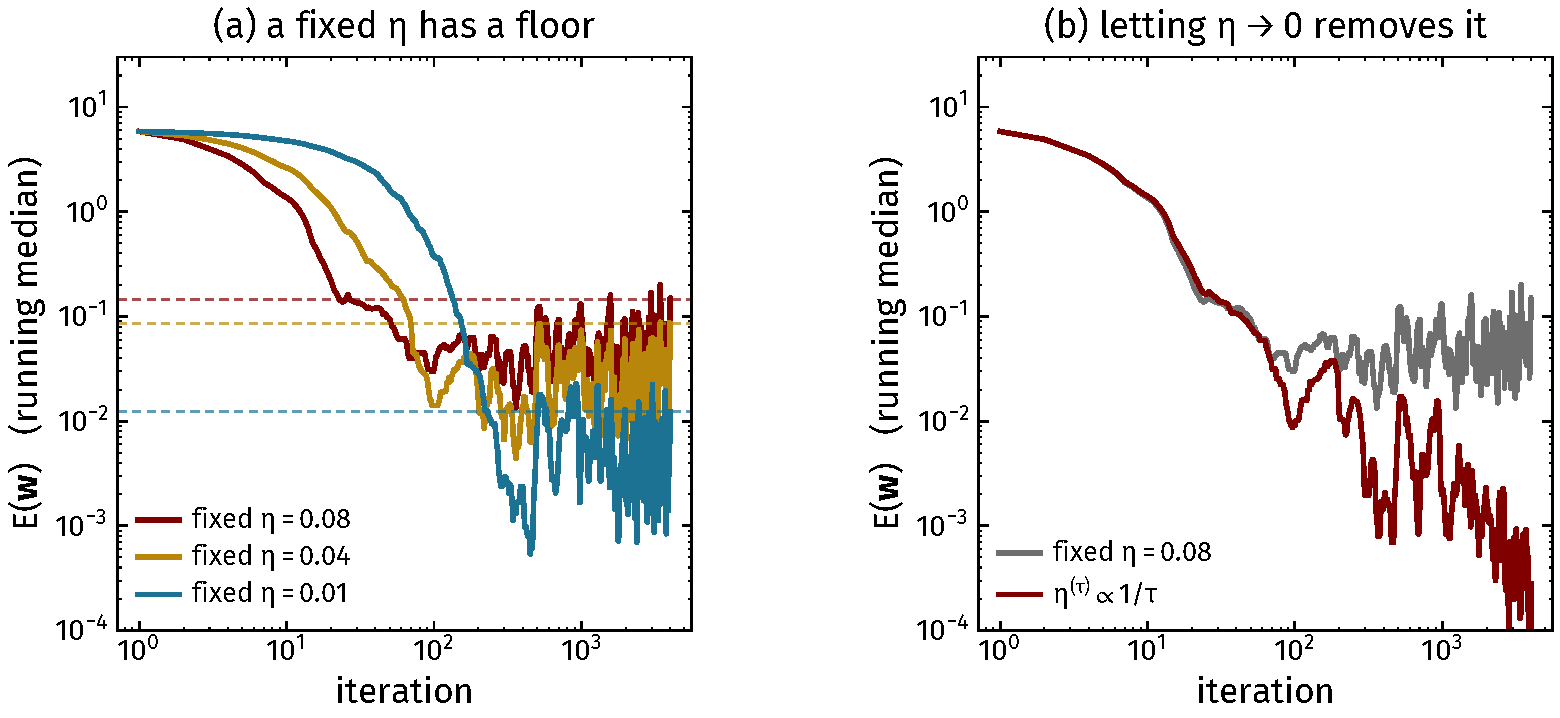
\includegraphics[height=0.58\textheight]{noise_floor}
  \end{center}
  \figcap[0.97]{(a) three fixed learning rates on the same noisy problem:
  each stops improving at a level proportional to $\eta$. (b) the same
  problem with $\eta$ decayed as $1/\tau$, which keeps descending past
  every one of those floors.}
\end{frame}

\begin{frame}{How fast may $\eta$ be allowed to fall?}
  \vspace{-0.35em}
  \begin{propx}[Robbins--Monro conditions]\label{th:rm}
    \small
    For stochastic (gradient descent) approximation with unbiased, bounded-variance
    gradients, the iterates converge to a stationary point provided
    $\sum_{\tau} \eta^{(\tau)} = \infty$ and
    $\sum_{\tau} \big(\eta^{(\tau)}\big)^{2} < \infty$.
  \end{propx}
  \vspace{0.3em}
  \begin{itemize}\itemsep0.3em
    \item The first says the steps must still be able to travel an
          unbounded distance: decay too fast and the iterate stalls
          before it arrives
    \item The second says the accumulated noise must be finite: decay
          too slowly and it never settles
    \item $\eta^{(\tau)} \propto 1/\tau$ satisfies both;
          $1/\sqrt{\tau}$ fails the second
  \end{itemize}
  \srcline{Robbins \& Monro (1951).}
\end{frame}

\begin{frame}{Three algebraic schedules}
  \vspace{0.2em}
  \begin{columns}[T, onlytextwidth]
    \begin{column}{0.33\textwidth}
      \centering \textbf{linear}\\[0.3em]
      $\eta^{(\tau)} = \big(1-\tfrac{\tau}{K}\big)\eta^{(0)}
        + \tfrac{\tau}{K}\eta^{(K)}$
    \end{column}
    \begin{column}{0.31\textwidth}
      \centering \textbf{power law}\\[0.3em]
      $\eta^{(\tau)} = \eta^{(0)}\big(1+\tfrac{\tau}{s}\big)^{-c}$
    \end{column}
    \begin{column}{0.33\textwidth}
      \centering \textbf{exponential}\\[0.3em]
      $\eta^{(\tau)} = \eta^{(0)}\, c^{\,\tau/s}$
    \end{column}
  \end{columns}
  \vspace{0.9em}
  \begin{itemize}\itemsep0.35em
    \item The linear form decays over $K$ steps and is then held at
          $\eta^{(K)}$
    \item $\eta^{(0)}$, $\eta^{(K)}$, $K$, $s$ and $c$ are found
          empirically
    \item Watching the learning curve is the practical test: it should
          be falling at a steady rate, not flattening early
  \end{itemize}
  \srcline{Bishop \& Bishop (2024), Eqs.~7.36--7.38.}
\end{frame}

\begin{frame}{The schedules in use}
  \begin{center}
    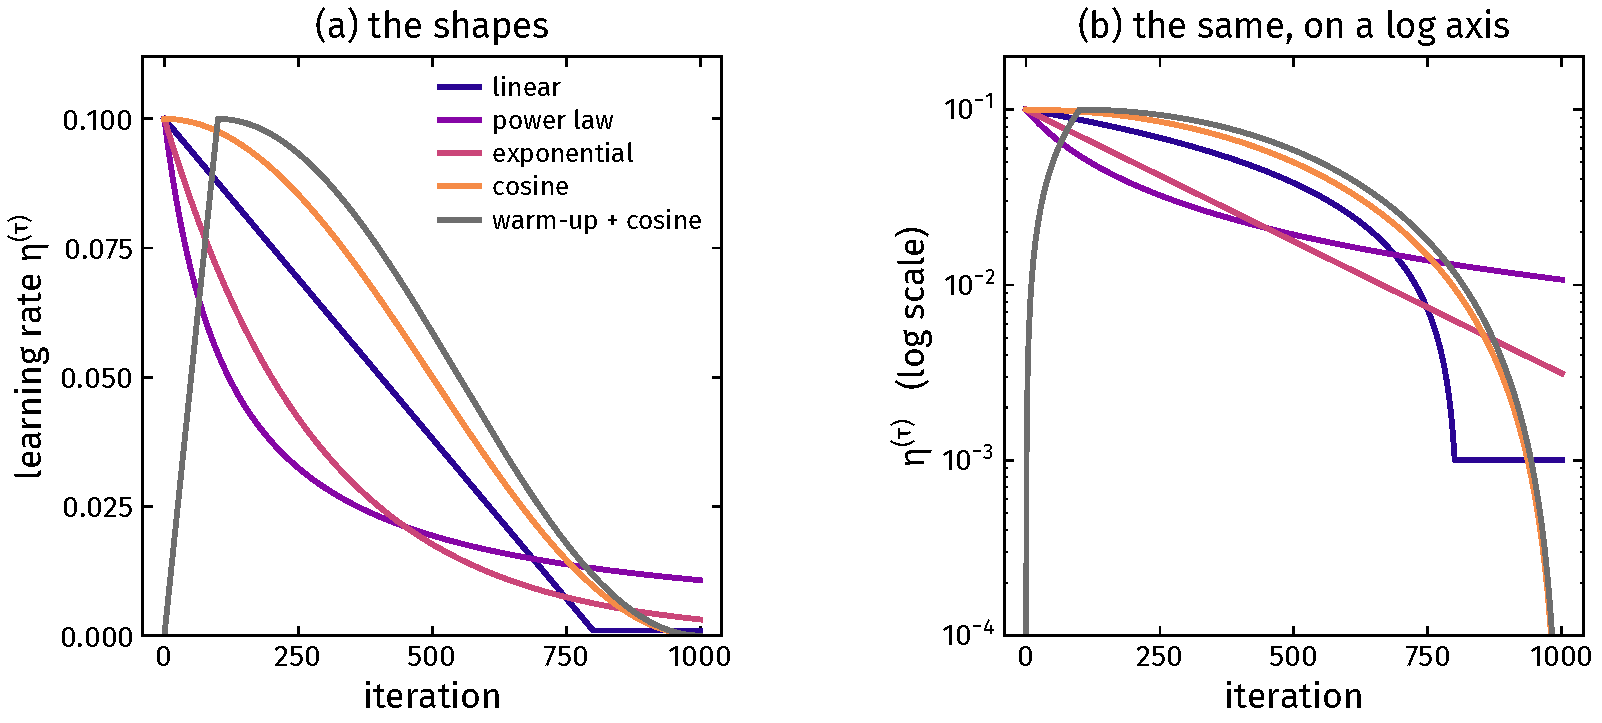
\includegraphics[height=0.58\textheight]{lr_schedules}
  \end{center}
  \figcap[0.97]{The three algebraic forms together with the two shapes
  most used in practice: cosine annealing, and a linear warm-up followed
  by cosine annealing.}
\end{frame}

\begin{frame}{Warm-up, and why the start is different}
  \vspace{0.3em}
  \begin{itemize}\itemsep0.45em
    \item Cosine annealing decays smoothly to zero over the whole run
          and has no schedule parameters to tune beyond its length
    \item \alert{Warm-up} raises $\eta$ from near zero over the first
          few thousand steps, then anneals
    \item The reason is that adaptive methods estimate gradient
          statistics from very few samples at the start, so those
          estimates are unreliable exactly when the steps are largest
    \item Warm-up is also standard when training with very large batches
  \end{itemize}
  \srcline{Loshchilov \& Hutter (2017); Goyal et al.~(2018).}
\end{frame}

% =====================================================================
\section{Adaptive Learning Rates}
% =====================================================================

\begin{frame}{One rate cannot serve two curvatures}
  \bridge{Momentum and schedules both keep a single $\eta$ shared by
  every parameter. That is the next assumption to drop.}
  \vspace{0.4em}
  \begin{itemize}\itemsep0.45em
    \item Gradient descent makes \alert{large} adjustments where the
          gradient is large --- where it should perhaps be cautious
    \item And \alert{small} adjustments where the gradient is small ---
          where it should perhaps explore
    \item If the surface is far steeper in one direction than another,
          no single $\eta$ makes good progress in both and stays stable
    \item The fix: give every parameter its own learning rate, adjusted
          automatically from what its gradients have been doing
  \end{itemize}
  \srcline{Prince (2023), \S6.4; Bishop \& Bishop (2024), \S7.3.3.}
\end{frame}



\begin{frame}{Normalising the gradient to its sign}
  \vspace{-0.3em}
  \[
    \mathbf{m}^{(\tau+1)} = \nabla E ,
    \qquad
    \mathbf{v}^{(\tau+1)} = \big(\nabla E\big)^{2} ,
    \qquad
    \mathbf{w}^{(\tau+1)} = \mathbf{w}^{(\tau)}
      - \eta\,\frac{\mathbf{m}^{(\tau+1)}}{\sqrt{\mathbf{v}^{(\tau+1)}} + \varepsilon}
  \]
  \vspace{-0.6em}
  \begin{itemize}\itemsep0.3em
    \item The root and the division are \alert{element-wise}, so every
          component reduces to its sign, and the step is a fixed
          distance $\eta$ along each axis
    \item $\varepsilon \sim 10^{-8}$ prevents division by zero
    \item It progresses in every direction and \alert{cannot converge}:
          it bounces around the minimum forever
  \end{itemize}
  \srcline{Prince (2023), Eqs.~6.13--6.14.}
\end{frame}

\begin{frame}{AdaGrad}
  \vspace{-0.3em}
  \[
    r^{(\tau)}_i = r^{(\tau-1)}_i
      + \left(\frac{\partial E}{\partial w_i}\right)^{2} ,
    \qquad
    \mathbf{w}^{(\tau)}_i = \mathbf{w}^{(\tau-1)}_i
      - \frac{\eta}{\sqrt{r_i} + \varepsilon}
        \left(\frac{\partial E}{\partial w_i}\right)
  \]
  \vspace{-0.6em}
  \begin{itemize}\itemsep0.3em
    \item Each parameter accumulates the sum of its own squared
          gradients, from $r^{(0)}_i = 0$
    \item Parameters that have seen large gradients --- high curvature
          --- have their rates reduced most
    \item \alert{The flaw}: $r_i$ accumulates from the first step and
          never forgets, so the steps eventually become too small and
          learning stalls
  \end{itemize}
  \srcline{Duchi, Hazan \& Singer (2011); Bishop \& Bishop (2024),
  Eqs.~7.39--7.40.}
\end{frame}

\begin{frame}{RMSProp}
  \vspace{-0.3em}
  \[
    r^{(\tau)}_i = \beta\, r^{(\tau-1)}_i
      + (1-\beta)\left(\frac{\partial E}{\partial w_i}\right)^{2} ,
    \qquad
    \mathbf{w}^{(\tau)}_i = \mathbf{w}^{(\tau-1)}_i
      - \frac{\eta}{\sqrt{r_i} + \varepsilon}
        \left(\frac{\partial E}{\partial w_i}\right)
  \]
  \vspace{-0.5em}
  \begin{itemize}\itemsep0.4em
    \item One change from AdaGrad: the running \emph{sum} becomes a
          running \emph{average}, with $0 < \beta < 1$ and typically
          $\beta = 0.9$
    \item The estimate now forgets on a timescale of about
          $1/(1-\beta)$ steps, so it tracks the curvature the iterate is
          currently in
    \item The learning rate can go back up when the surface flattens,
          which is exactly what AdaGrad could not do
  \end{itemize}
  \srcline{Hinton (2012); Bishop \& Bishop (2024), Eqs.~7.41--7.42.}
\end{frame}

\begin{frame}{Adam}
  \vspace{-0.55em}
  \begin{columns}[T, onlytextwidth]
    \begin{column}{0.485\textwidth}
      \[ s^{(\tau)}_i = \beta_1 s^{(\tau-1)}_i
         + (1-\beta_1)\frac{\partial E}{\partial w_i} \]
    \end{column}
    \begin{column}{0.50\textwidth}
      \[ r^{(\tau)}_i = \beta_2 r^{(\tau-1)}_i
         + (1-\beta_2)\left(\frac{\partial E}{\partial w_i}\right)^{2} \]
    \end{column}
  \end{columns}
  \vspace{-0.55em}
  \begin{columns}[T, onlytextwidth]
    \begin{column}{0.30\textwidth}
      \[ \hat s_i = \frac{s^{(\tau)}_i}{1-\beta_1^{\tau}} \]
    \end{column}
    \begin{column}{0.30\textwidth}
      \[ \hat r_i = \frac{r^{(\tau)}_i}{1-\beta_2^{\tau}} \]
    \end{column}
    \begin{column}{0.38\textwidth}
      \[ \mathbf{w}^{(\tau)}_i = \mathbf{w}^{(\tau-1)}_i
         - \frac{\eta\,\hat s_i}{\sqrt{\hat r_i} + \varepsilon} \]
    \end{column}
  \end{columns}
  \vspace{0.1em}
  \begin{itemize}\itemsep0.3em
    \item RMSProp with momentum: an exponential average of the gradient
          \emph{and} of its square. The name is short for
          \alert{adaptive moment estimation}
    \item Typical values are $\beta_1 = 0.9$ and $\beta_2 = 0.99$
    \item The most widely used training algorithm in deep learning
  \end{itemize}
  \srcline{Kingma \& Ba (2015); Bishop \& Bishop (2024),
  Eqs.~7.43--7.47.}
\end{frame}

\begin{frame}{Why the bias correction is required?}
  \vspace{-0.25em}
  \begin{propx}[Biased Estimates]\label{th:bias}
    \small
    With $\mathbf{s}^{(0)} = 0$ and a gradient $\mathbf{g}$ that is constant in
    expectation,
    \[
      \mathbb{E}\big[\mathbf{s}^{(\tau)}\big]
        = \big(1 - \beta_1^{\tau}\big)\, \mathbf{g} ,
    \]
    so $\mathbf{s}^{(\tau)}$ underestimates $\mathbf{g}$ by exactly the factor
    $1 - \beta_1^{\tau}$. Dividing by that factor removes the bias, and
    since $\beta_1 < 1$ the correction tends to one as $\tau$ grows.
  \end{propx}
  \vspace{0.05em}
  {\footnotesize
  \begin{itemize}\itemsep0.26em
    \item \focus{1}{Unrolling gives
          $\mathbf{s}^{(\tau)} = (1-\beta_1)\sum_{k=0}^{\tau-1}\beta_1^{k}
          \mathbf{g}^{(\tau-k)}$.}
    \item \focus{1}{Taking expectations and summing the geometric series
          gives $(1-\beta_1)\frac{1-\beta_1^{\tau}}{1-\beta_1} \mathbf{g}$.}
    \item \focus{1}{Dividing by $1-\beta_1^{\tau}$ therefore returns $\mathbf{g}$
          exactly; the same argument applies to $r$ with $\beta_2$.
          \hfill $\square$}
  \end{itemize}}
  \vspace{-0.3em}
  \srcline{Bishop \& Bishop (2024), Eqs.~7.45--7.46; Prince (2023),
  Eq.~6.16.}
\end{frame}

\begin{frame}{The correction, drawn}
  \begin{center}
    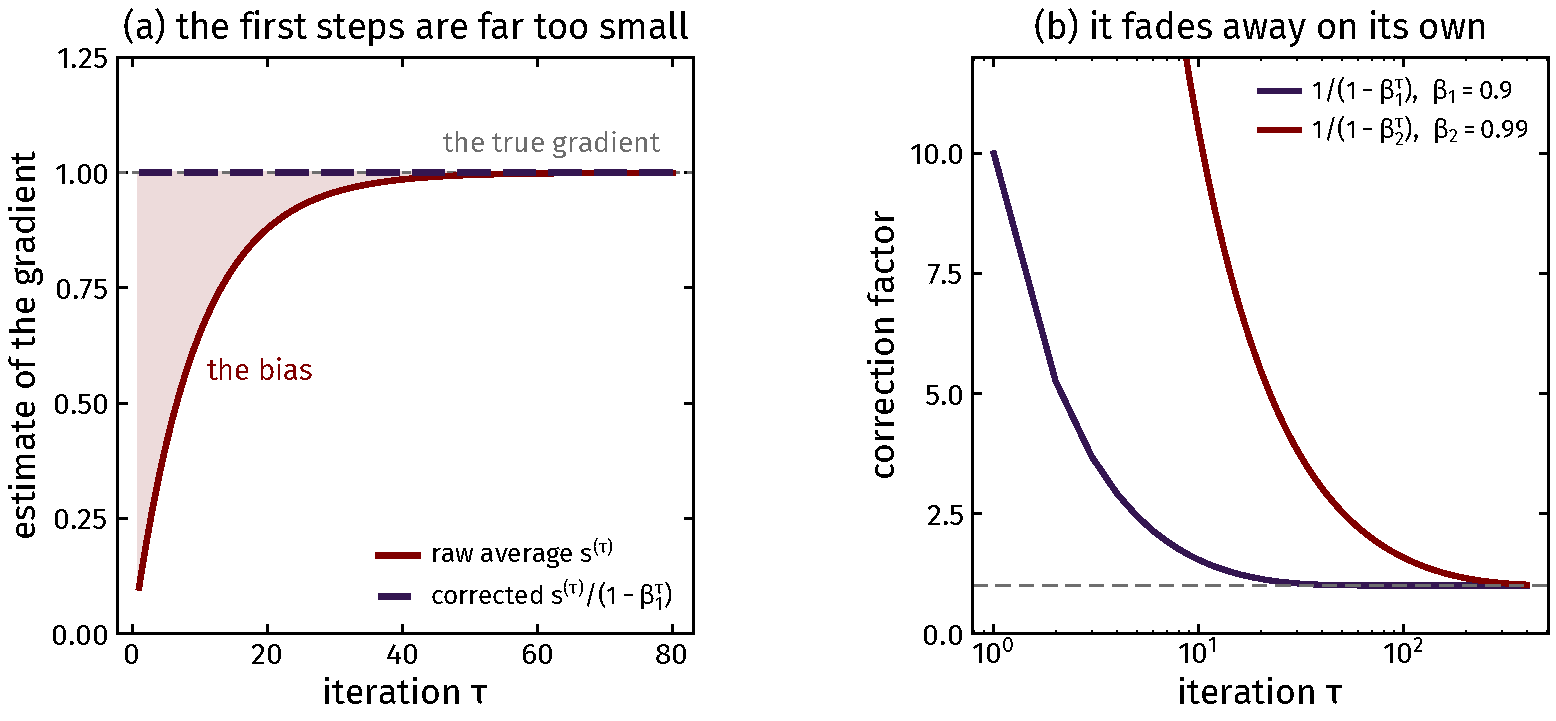
\includegraphics[height=0.545\textheight]{bias_correction}
  \end{center}
  \figcap[0.97]{(a) the running average of a constant gradient, with and
  without the correction. (b) the size of the correction factor against
  the iteration, for both decay parameters.}
\end{frame}

% \begin{frame}{Adam, as an algorithm}
%   \vspace{0.15em}
%   \begin{algox}[Adam optimization]\label{th:algadam}
%     \small
%     \textbf{Input:} batch size $B$; per-batch error $E_{n:n+B-1}$;
%     learning rate $\eta$; decay parameters $\beta_1, \beta_2$;
%     stabilizer $\varepsilon$\\[0.3em]
%     $\mathbf{s} \leftarrow 0$; \quad $\mathbf{r} \leftarrow 0$; \quad $\tau \leftarrow 0$\\
%     \textbf{repeat}\\
%     \hspace{1.2em} choose a mini-batch at random; \quad
%       $\mathbf{g} \leftarrow \nabla E_{n:n+B-1}(\mathbf{w})$; \quad
%       $\tau \leftarrow \tau + 1$\\
%     \hspace{1.2em} $\mathbf{s} \leftarrow \beta_1 \mathbf{s} + (1-\beta_1) \mathbf{g}$; \quad
%       $\mathbf{r} \leftarrow \beta_2 \mathbf{r} + (1-\beta_2)\, \mathbf{g} \odot \mathbf{g}$
%       \hfill \textcolor{mcMuted}{// element-wise}\\
%     \hspace{1.2em} $\hat{\mathbf{s}} \leftarrow \mathbf{s}/(1-\beta_1^{\tau})$; \quad
%       $\hat{\mathbf{r}} \leftarrow \mathbf{r}/(1-\beta_2^{\tau})$
%       \hfill \textcolor{mcMuted}{// bias correction}\\
%     \hspace{1.2em} $\mathbf{w} \leftarrow \mathbf{w}
%       - \eta\,\hat{\mathbf{s}} / (\sqrt{\hat{\mathbf{r}}} + \varepsilon)$
%       \hfill \textcolor{mcMuted}{// element-wise}\\
%     \textbf{until} convergence; \quad \textbf{return} $\mathbf{w}$
%   \end{algox}
%   \srcline{Bishop \& Bishop (2024), Algorithm 7.4.}
% \end{frame}

\begin{frame}{Five update rules, by family}
  \begin{center}
    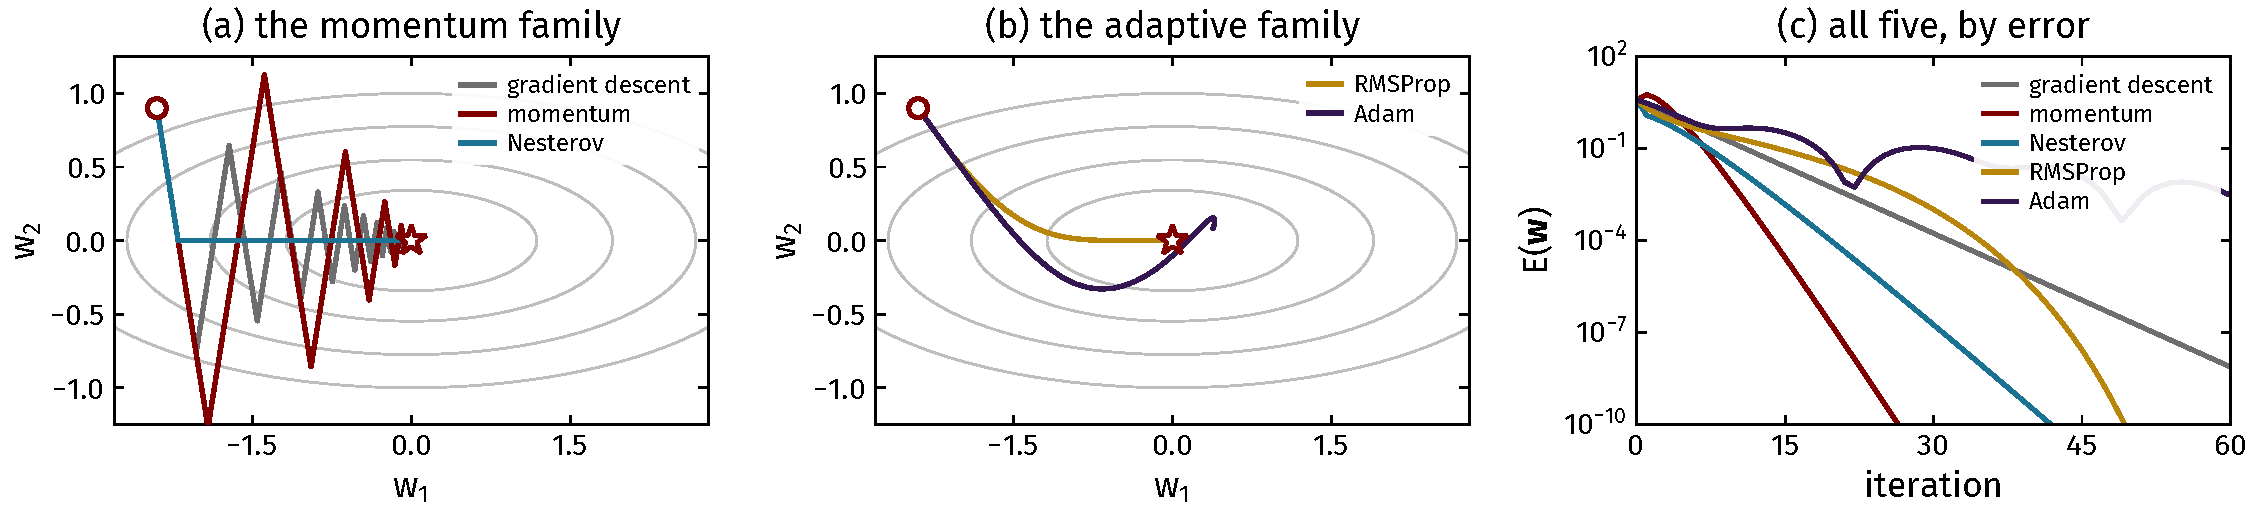
\includegraphics[width=0.94\linewidth]{optimiser_compare}
  \end{center}
  \figcap[0.97]{The same ill-conditioned quadratic and start throughout,
  each method at constants that suit it. (a) the momentum family attacks
  the ratio $\lambda_{\max}/\lambda_{\min}$, and still crosses the
  valley. (b) the adaptive family rescales each coordinate instead, and
  turns along the floor rather than across it.}
\end{frame}

% \begin{frame}{What the five cost}
%   \begin{center}
%     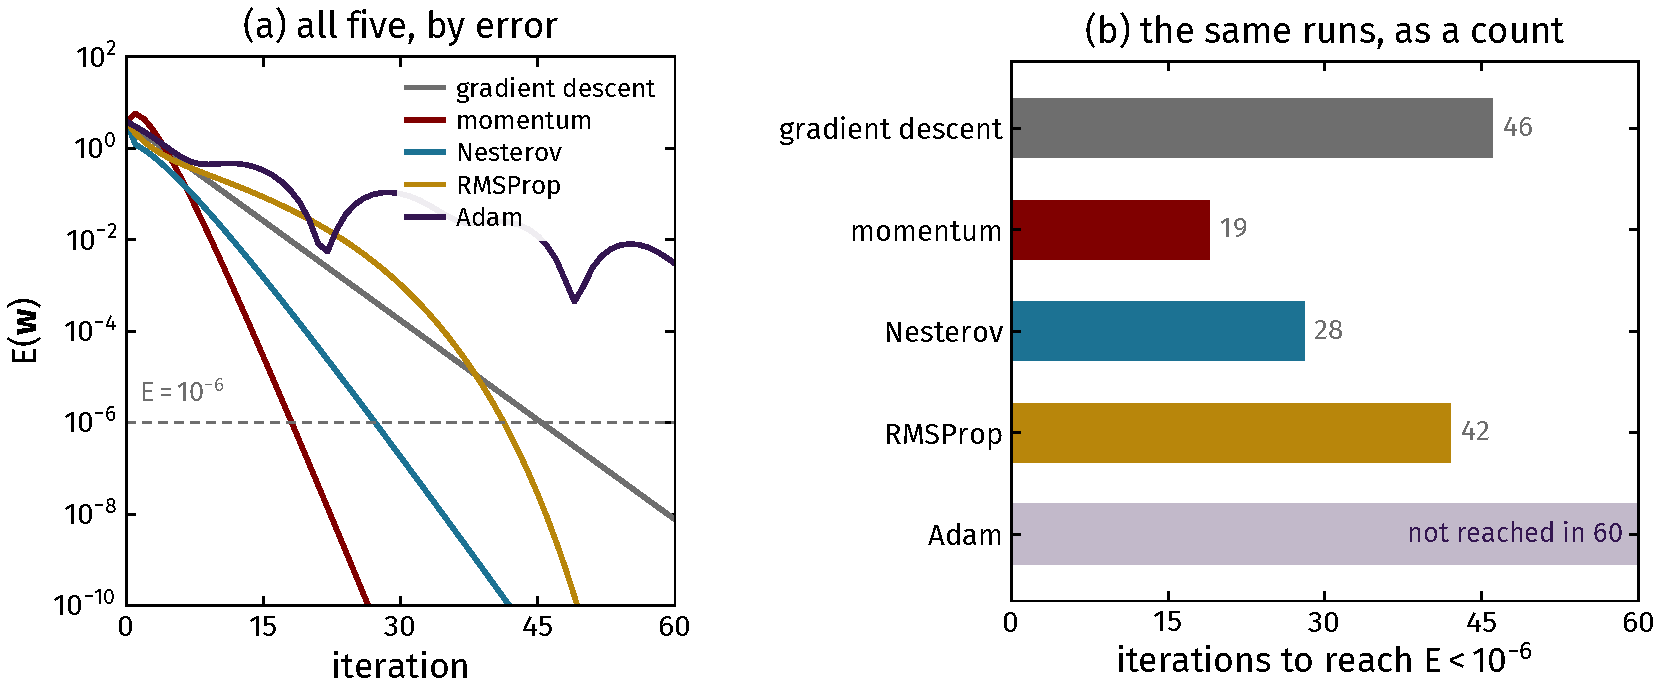
\includegraphics[width=0.80\linewidth]{optimiser_cost}
%   \end{center}
%   \figcap[0.97]{(a) the same five runs by error. (b) iterations needed to
%   reach $E < 10^{-6}$; Adam does not get there inside the budget. Why the
%   families differ matters more than the ordering on any one surface.}
% \end{frame}

\begin{frame}{Four honest caveats}
  \begin{itemize}\itemsep0.3em
    \item The per-parameter argument assumes the principal curvature
          directions are \alert{aligned with the axes} of weight space
          --- a diagonal Hessian, which is unlikely. The methods work
          anyway
    \item Adam's original convergence proof was for convex losses;
          Reddi et al.~(2018) exhibited a counterexample and proposed
          AMSGrad, which does converge
    \item Adam interacts badly with $L^2$ regularization; AdamW
          separates the two and is the common default
    \item Evidence runs in both directions on whether SGD with momentum
          generalizes better than Adam; much of the gap disappears once
          Adam's hyperparameters are tuned
  \end{itemize}
  \srcline{Prince (2023), Notes to Ch.~6.}
\end{frame}

% =====================================================================
\section{Putting It Together}
% =====================================================================

\begin{frame}{What each method actually fixes}
  \vspace{0.3em}
  {\footnotesize
  \renewcommand{\arraystretch}{1.38}
  \begin{tabular}{@{}l@{\hspace{1.3em}}l@{\hspace{1.3em}}l@{}}
    \textbf{Method} & \textbf{Attacks} & \textbf{Contraction factor}\\
    gradient descent & --- & $(\kappa-1)/(\kappa+1)$\\
    momentum & the condition number &
      $(\sqrt{\kappa}-1)/(\sqrt{\kappa}+1)$\\
    Nesterov momentum & the condition number & $1 - 1/\sqrt{\kappa}$\\
    schedules & the gradient noise & removes the floor\\
    RMSProp, Adam & unequal curvature per parameter & no clean bound\\
    normalization (Class 15) & $\kappa$ itself & changes the problem\\
  \end{tabular}}
  \vspace{0.65em}

  \begin{redhighlight}
    The first four change the \emph{iteration} and leave the surface
    alone. Only the last changes the surface --- which is why it is the
    subject of the next class.
  \end{redhighlight}
\end{frame}

\begin{frame}{The hyperparameters of the training algorithm}
  \vspace{0.35em}
  {\footnotesize
  \renewcommand{\arraystretch}{1.40}
  \begin{tabular}{@{}l@{\hspace{1.5em}}l@{\hspace{1.5em}}l@{}}
    \textbf{Choice} & \textbf{Typical} & \textbf{What it trades}\\
    optimizer & Adam, or SGD with momentum & speed against final quality\\
    learning rate $\eta$ & $10^{-3}$ (Adam), $10^{-1}$ (SGD) &
      stability against progress\\
    schedule & cosine, with warm-up & exploration against refinement\\
    momentum $\mu$ & $0.9$ & smoothing against responsiveness\\
    $\beta_1, \beta_2$ & $0.9$, $0.99$ & as above, per parameter\\
    batch size $B$ & a power of two & noise against cost (Class 13)\\
  \end{tabular}}
  \vspace{0.6em}

  \begin{itemize}\itemsep0.3em
    \item These belong to the \alert{algorithm}, not to the model, and
          are usually chosen by training several models and comparing on
          held-out data
  \end{itemize}
  \srcline{Prince (2023), \S6.5.}
\end{frame}

\begin{frame}{Takeaways}
  \vspace{0.15em}
  \vspace{-0.15em}
  {\footnotesize
  \begin{enumerate}\itemsep0.30em
    \item On a quadratic the eigen-directions contract independently by
          $(1-\eta\lambda_i)$, so one $\eta$ must serve every curvature
          at once (Lemma~\ref{th:decay})
    \item Stability is set by $\lambda_{\max}$ and speed by
          $\lambda_{\min}$; with equal curvature one step suffices
    \item The condition number $\kappa$ measures the gap, and the number
          of steps is proportional to it (Proposition~\ref{th:opt})
    \item Momentum accelerates along a consistent slope by
          $1/(1-\mu)$ and cancels across an oscillating one
          (Proposition~\ref{th:mom}), replacing $\kappa$ by
          $\sqrt{\kappa}$
    \item A fixed $\eta$ leaves a noise floor; a schedule satisfying
          $\sum\eta = \infty$, $\sum\eta^2 < \infty$ removes it
          (Proposition~\ref{th:rm})
    \item Adaptive methods give each parameter its own rate from its
          own gradient history; Adam is RMSProp with momentum and a
          bias correction
  \end{enumerate}}
  \vspace{0.2em}
  \bridge{Next class: rather than repairing the iteration, we rescale
  the network so that $\kappa$ is small to begin with.}
\end{frame}

\begin{frame}{References}
  \vspace{0.2em}
  {\scriptsize
  \begin{itemize}\itemsep0.26em
    \item C.~M. Bishop \& H. Bishop, \emph{Deep Learning: Foundations
          and Concepts}, Springer, 2024. \S7.3 (Eqs.~7.24--7.47,
          Algorithms 7.3--7.4, Figs.~7.3--7.6).
    \item S.~J.~D. Prince, \emph{Understanding Deep Learning}, MIT
          Press, 2023. \S6.3--6.5 (Eqs.~6.11--6.18, Figs.~6.7--6.9).
    \item B.~T. Polyak, ``Some methods of speeding up the convergence of
          iteration methods'', \emph{USSR Comp.~Math.}, 1964.
    \item Y. Nesterov, ``A method for solving the convex programming
          problem with convergence rate $O(1/k^2)$'', 1983.
    \item H. Robbins \& S. Monro, ``A stochastic approximation method'',
          \emph{Ann.~Math.~Statist.}, 1951.
    \item J. Duchi, E. Hazan \& Y. Singer, ``Adaptive subgradient
          methods'', \emph{JMLR}, 2011.
    \item D.~P. Kingma \& J. Ba, ``Adam: a method for stochastic
          optimization'', \emph{ICLR}, 2015.
    \item S.~J. Reddi, S. Kale \& S. Kumar, ``On the convergence of Adam
          and beyond'', \emph{ICLR}, 2018.
    \item I. Loshchilov \& F. Hutter, ``SGDR'', \emph{ICLR}, 2017;
          ``Decoupled weight decay regularization'', \emph{ICLR}, 2019.
  \end{itemize}}
\end{frame}

\begin{frame}[standout]
  Questions?
\end{frame}
\begin{frame}{The problem, and three responses}
  \begin{center}
    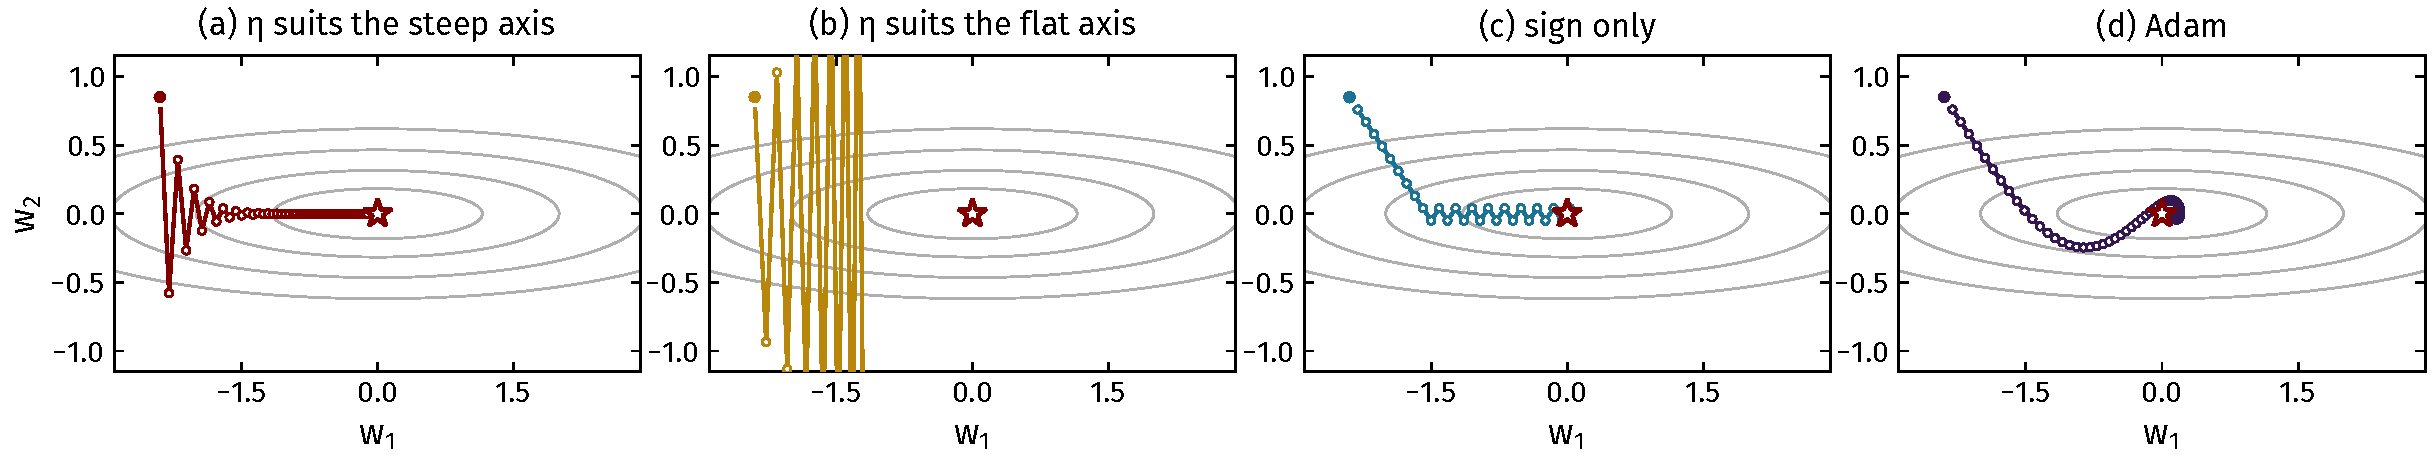
\includegraphics[width=0.99\linewidth]{per_parameter}
  \end{center}
  \figcap[0.98]{(a) an $\eta$ chosen for the steep direction leaves the
  flat one barely moving. (b) an $\eta$ chosen for the flat direction is
  unstable. (c) using only the sign of each component moves a fixed
  distance along each axis, and makes progress in both, but cannot
  settle. (d) Adam smooths both quantities and does settle.}
\end{frame}
\end{document}
